\documentclass{beamer}

\usepackage{etoolbox}
\usepackage{graphicx}
\usepackage{enumerate}
\usepackage{verbatim}
\usepackage{tikz}
\newcommand{\HAT}[1]{\expandafter\hat#1}

\usetheme{Frankfurt}%
\usecolortheme{beaver}
%\logo{
\includegraphics[height=.125in]{img/ugaLogo}}

% %%%%%%%%%%%%%%%%%%%%%%%%%%%%%%%%%%%%%%%%%%%%%%%%%%%%%%%%%%%%%%%%%%%%%%%
% List of definitions that are used in the different pages for the
% notes

% %%%%%%%%%%%%%%%%%%%%%%%%%%%%%%%%%%%%%%%%%%%%%%%%%%%%%%%%%%%%%%%%%%%%%%%
% Basic definitions used throughout the notes

\newcommand{\half}{\mbox{$\frac{1}{2}$}}
\newcommand{\deltat}{\mbox{$\triangle t$}}
\newcommand{\deltax}{\mbox{$\triangle x$}}
\newcommand{\deltay}{\mbox{$\triangle y$}}

\newcommand{\deriv}[2]{\frac{d}{d#2}#1}
\newcommand{\derivTwo}[2]{\frac{d^2}{d#2^2}#1}

\newcommand{\lp}{\left(}
\newcommand{\rp}{\right)}


% %%%%%%%%%%%%%%%%%%%%%%%%%%%%%%%%%%%%%%%%%%%%%%%%%%%%%%%%%%%%%%%%%%%%%%
% Basic color additions
\definecolor{fuchsia}{RGB}{255,0.0,255}
\definecolor{georgiaRed}{RGB}{100,0,00}
\definecolor{light-gray}{gray}{0.8}
\definecolor{mediumGray}{gray}{0.6}


\newcommand{\redText}[1]{{\color{red}#1}}
\newcommand{\blueText}[1]{{\color{blue}#1}}
\newcommand{\greenText}[1]{{\color{green}#1}}
\newcommand{\fuchsiaText}[1]{{\color{fuchsia}#1}}


%%% Local Variables:
%%% mode: latex
%%% TeX-master: "Presentation1"
%%% End:




\setbeamercolor{palette primary}{fg=georgiaRed,bg=white}
\setbeamercolor{palette secondary}{fg=georgiaRed,bg=white}
\setbeamercolor{palette tertiary}{fg=georgiaRed,bg=white}
\setbeamercolor{palette quaternary}{bg=mediumGray,fg=black}
\setbeamercolor{block title}{fg=black,bg=black!15}
\setbeamercolor{block body}{fg=black,bg=black!10}
\setbeamercolor{titlelike}{bg=georgiaRed,fg=black} % parent=palette quaternary}


\setbeamercolor{upper separation line head}{bg=red}
\setbeamercolor{headline}{bg=red}
\setbeamertemplate{headline}
{%
\begin{beamercolorbox}{section in head/foot}
\insertsectionnavigationhorizontal{.75\textwidth}{}{}
\hfill \insertpagenumber /\insertdocumentendpage
\end{beamercolorbox}%
}
\setbeamercolor{section number projected}{bg=red,fg=black}
\setbeamercolor{subsection number projected}{bg=red,fg=black}
%\setbeamercolor{frametitle}{bg=lightgray,fg=black}



\begin{document}

\author{Valerie A. Carrasquillo, Claudia L. Guerrero, Michael M. Law, and Kyle McGrath}
\institute{Universidad Metropolitana, Universidad Autónoma del Estado de Hidalgo, University of Florida, and
  SUNY-Potsdam}

\title{Making Corals Come To Life}
\subtitle{Adventures In Stochastic Differential Equations}
\date{June 12, 2015.}

\begin{frqame}
  \titlepage
\end{frame}

\begin{frame}
  \frametitle{Outline}
  \tableofcontents
\end{frame}

%<<<<<<< HEAD

\section{Biological background}

\begin{frame}
\frametitle{Coral Reef}
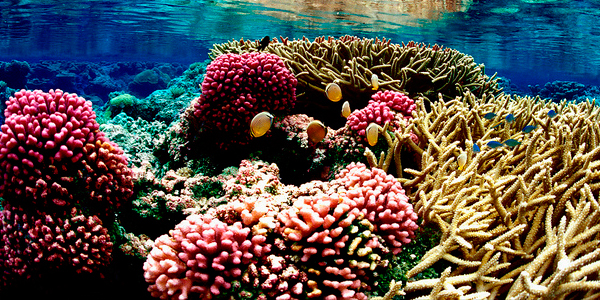
\includegraphics[scale=.175]{./US-Wildlife-coral-1.jpg}
\begin{itemize}
\item A complex aquatic ecosystem physically supported by calcium carbonate secretions of the colorful stone coral.
\item Modeling approach by Li-Wang-Zhang-Hastings is to describe the relationships between macroalgae, algal turfs, and corals (Li et al., 2014).
\end{itemize}
\end{frame}

\begin{frame}
\frametitle{Positives}
\begin{itemize}
\item Macroalgae naturally filter the water by reducing the levels of phosphate and nitrogenous waste.
\item Macroalgae provide hiding places for fishes and invertebrates
\item Macroalgae convert energy into food for the rest of the reef food web
\end{itemize}
\end{frame}

\begin{frame}
\frametitle{Coral Reef Ecosystem} 

McClanahan (1994) identifies three major components:
\begin{itemize}
\item Primary producers (coral and algae)\\
\item Herbivores (e.g. scarid grazing)\\
\item Carnivores
\end{itemize}
\end{frame}

\begin{frame}
\centering
\frametitle{Reef Food Web}
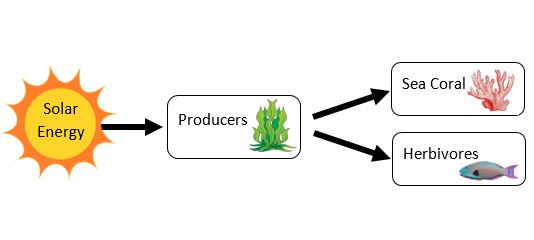
\includegraphics[scale=.65]{./CoralFoodWeb}
\end{frame}

\begin{frame}
\frametitle{Negatives}
\begin{itemize}
\item At low grazing levels, the macroalgal population increases and competes with the coral population for space.
\item This competition alters the microbial communities associated with corals increasing pathogens on corals.
\item Macroalgal abundance may lead to reef degradation.
\item Coral mortality is generally followed by algal recruitment.
\end{itemize}
\end{frame}

\begin{frame}
\frametitle{Coral Reef Dynamics}
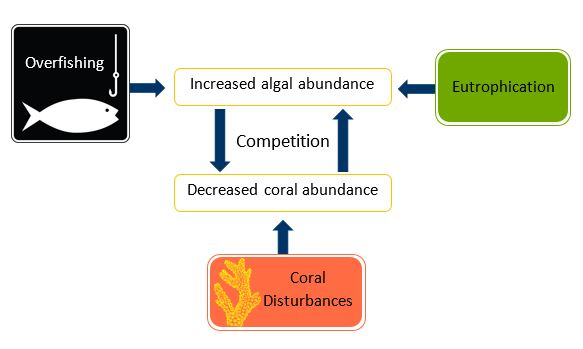
\includegraphics[scale=.7]{./CoralDynamics}
\end{frame}


\section{Brownian Motion}

\begin{frame}{Brownian motion}
Brownian motion can be constructed as a limit of random walks.
\begin{eqnarray*}
 P(Y_i=\Delta x)=\frac{1}{2} \\
 P(Y_i=-\Delta x)=\frac{1}{2}
\end{eqnarray*}
\pause

\begin{center}
What is the distribution of 
\begin{equation*}
X_n=Y_1+Y_2+...+Y_n
\end{equation*}
if $Y_1,Y_2,...,Y_n$ are i.i.d.? 
\end{center}
\end{frame}


\begin{frame}
\begin{eqnarray*}
X_n&= &Y_1+Y_2+...+Y_n\\ \\
\pause
\ln (M_{X_n})(\lambda)&\approx &\frac{(\Delta x)^2}{\Delta t} \left(\frac{\lambda ^2 T}{2}+\frac{\lambda ^4 \Delta x ^2 T}{4}+... \right)\\
\end{eqnarray*}
\pause
If we assume that $\frac{(\Delta x)^2}{\Delta t}=k$ then,
\begin{equation*}
\lim_{\Delta x \to 0}{M_{X_n}(\lambda)}=\exp\left(\frac{kT\lambda ^2}{2}\right)
\end{equation*}
which means $X_n \sim N(0,kT)$
\end{frame}

\begin{frame}
\begin{block}{Standard Brownian Motion}
A random variable $B(t)$ that depends continuously on $t \in [0,T]$ and satisfies: 
\begin{itemize}
\item $B(0)=0$
\item For $0 \leq s<t\leq T$: $B(t)-B(s)\sim N(0, t-s)$
\item For $0 \leq s<t<u<v\leq T$ the increments $B(t)-B(s)$ and $B(v)-B(u)$ are independent.
\end{itemize}
\end{block}
\end{frame}

\begin{frame}{Computational Purposes}
Discretized Brownian motion: $B(t)$ is specified at discrete t values.
\begin{eqnarray*}
&& W(0)=0\\
&& W(j)=W(j-1)+dW(j)
\end{eqnarray*}
$dW(j)$ is an independent random variable of the form $N(0,\Delta t)$
\end{frame}

\begin{frame}
\begin{center}
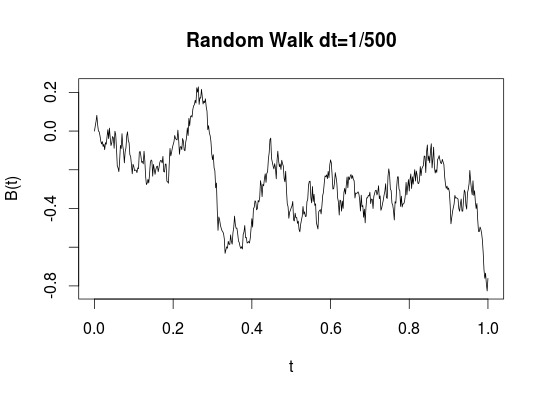
\includegraphics[scale=0.5]{r_w_3.png}
\end{center}
\end{frame}

\begin{frame}
\begin{center}
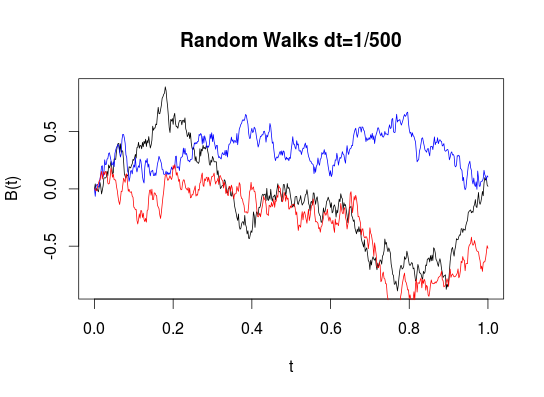
\includegraphics[scale=0.5]{r_w_4.png}
\end{center}
\end{frame}

\begin{frame}
\begin{center}
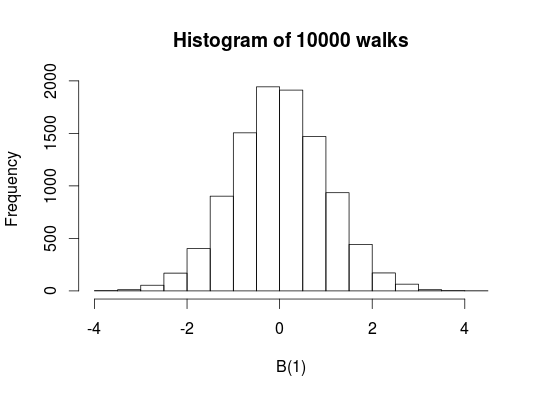
\includegraphics[scale=0.5]{hist.png}
\end{center}
\end{frame}

\begin{frame}
\begin{center}
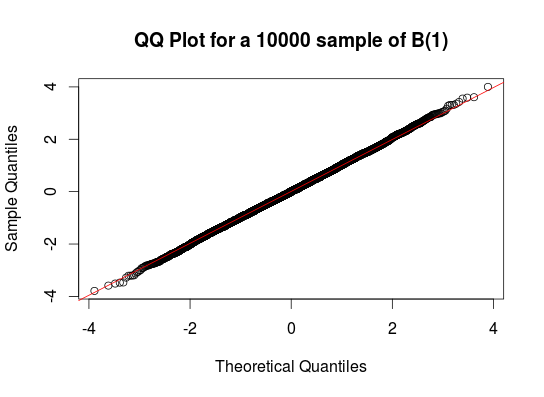
\includegraphics[scale=0.5]{qqplot.png}
\end{center}
\end{frame}


\section{Stochastic Integrals}

\begin{frame}{Stochastic Integrals}
\pause
\begin{center}
What does $\int_{a}^{b} f(t)dB$ mean? \bigskip \pause  $\int_{a}^{b} B(t)dB$?\pause \\

¿An analogy of the Riemann-Stietjes sum?\\ \pause 
%\begin{equation*}
%\sum_{i=1}^{n}B(t_{j-1})\left( B(t_{j})-B(t_{j-1})\right) 
%\end{equation*}
%\pause
\bigskip

In $[0,T]$ with $\Delta t=1/500$:\\ \pause
$It\hat{o}=-0.42765$\\ \pause
$Stratonovich=0.088892$
\end{center}
\end{frame}

%\begin{frame}
%Consider the following functions:
%\[1_{[t_{i-1},t_i)} = \left \{
%  \begin{array}{lr}
%1, & t \in [t_{i-1},t_i)\\
%0, & otherwise
%  \end{array}
%\right.
%\]

%$$f_n=\sum_{i=1}^{n}a_i1_{[t_{i-1},t_i)} $$\\

%We define the stochastic integral as:
%$$I(f_n):=\sum_{i=1}^{n} a_i(B(t_i)-B(t_{i-1}))$$
%\end{frame}

\begin{frame}
\begin{block}{Definition}
Given f(t) a continuous function with bounded variation. Let $a_i=f(t_{i-1})$, then \textbf{the Weiner integral} is:
\begin{equation*}
I(f):=\lim_{n \to \infty}\sum_{i=1}^{n}a_i(B(t_i)-B(t_{i-1}))
\end{equation*}
\pause
\begin{itemize}
\item $E[I(f)]=0$
\item $Var[I(f)]=\int_{a}^{b}f^2(t)dt$
\end{itemize}
\end{block}

%\begin{eqnarray*}
%E[I(f)]&=&0\\
%Var[I(f)]&=&\int_{a}^{b}f^2(t)dt
%\end{eqnarray*}
\end{frame}

\section{It\^o's Formulas}

%\begin{frame}
%  \frametitle{Differentiation and Integration of Stochastic Processes}
%
%  \begin{itemize}
%   \item Brownian motion is a continuous time stochastic process that is nowhere differentiable.\\
%  \item  How do we make sense of $\frac{dB}{dt}$?\\
%\end{itemize}
%
%\end{frame}

\begin{frame}
  \frametitle{Riemann-Stieltjes Integration of Stochastic Processes}
  \begin{itemize}
  \item Riemann-Stieltjes Integral \\
    $$\int_{a}^{b} f(x) d\alpha(x)=\lim_{n\to\infty}\sum_{i=1}^{n} f(x_i) (\alpha(x_i)-\alpha(x_{i-1}))$$\\
  \item  Stochastic Integral \\
    $$\int_{a}^{b} f(t) dB=\lim_{n\to\infty}\sum_{i=1}^{n} f(t_{i-1}) (B(t_i)-B(t_{i-1}))$$\\
  %\item  Form the Taylor expansion on $f(B(b))-f(B(a))$\\
  \end{itemize}
\end{frame}


\begin{frame}
  \frametitle{Left and Right Riemann-Stieltjes Sums}
  \begin{itemize}
  \item Left Side Riemann-Stieltjes sum $$L=\lim_{n\to\infty}\sum_{i=1}^{n} f(t_{i-1}) (B(t_i)-B(t_{i-1}))$$\\
  \item Right Side Riemann-Stieltjes sum $$R=\lim_{n\to\infty}\sum_{i=1}^{n} f(t_i) (B(t_i)-B(t_{i-1}))$$\\

  \end{itemize}
\end{frame}
  
\begin{frame}
  \frametitle{Left and Right Riemann-Stieltjes Sums}
  \begin{itemize}
  \item Considering $$\int_{a}^{b}{B(t)d(B(t))}$$\\
  \item The left sided limit \\
    $$L=\frac{1}{2}B^2(t)-\frac{t}{2}$$\\
  \item The right sided limit \\
    $$R=\frac{1}{2}B^2(t)+\frac{t}{2}$$\\
  \end{itemize}  
\end{frame}
  
\begin{frame}
  \frametitle{It\^{o}'s Formula (First Formulation)}
  \begin{itemize}
  \item $\Delta B^2 \to \Delta t$\\
  \item  The Taylor expansion is
  \begin{eqnarray*}
    f(B(t_i))-f(B(t_{i-1}))&=&f'(B(t_{i-1}))(B(t_i)-B(t_{i-1}))+\\
    & &\frac{1}{2}f''(B(t_{i-1}))(B(t_i)-B(t_{i-1}))^2+\\
    %& &\frac{1}{3}f'''(B(t_{i-1}))(B(t_i)-B(t_{i-1}))^3+\\
    & &\mathrm{Higher Order Terms}\\
  \end{eqnarray*}
  %f(B(b))-f(B(a))&=&\sum_{i=1}^{n}(f'(B(t_{i-1}))(B(t_i)-B(t_{i-1}))+\\
  %& &\frac{1}{2}f''(B(t_{i-1}))(B(t_i)-B(t_{i-1}))^2+\\
  %& &\frac{1}{3}f'''(B(t_{i-1}))(B(t_i)-B(t_{i-1}))^3+\\
  %& &\mathrm{Higher Order Terms})\\
  \item Taking the sum of the telescoping series $$f(B(b))-f(B(a))=\sum_{i=1}^{n}(f(B(t_i))-f(B(t_{i-1})))$$\\
  \item It\^o's Formula (first version) $$f(B(b))-f(B(a))=\int_{a}^{b}{\frac{\partial f}{\partial B} dB}+\int_{a}^{b}{\frac{1}{2} \frac{\partial^2 f}{\partial B^2} dt} $$\\
  \end{itemize}
\end{frame}

\begin{frame}
  \frametitle{It\^o's Formula (Second and Third Formulation)}
  \begin{itemize}
  \item  It\^o's Formula (second version) $$f(b,B(b))-f(a,B(a))=\int_{a}^{b}{\frac{\partial f}{\partial B} dB}+\int_{a}^{b}{(\frac{\partial f}{\partial s}+\frac{1}{2}\frac{\partial ^2 f}{\partial B^2}) ds}$$\\
  \item  It\^o's Formula (third version): The Stochastic Chain Rule $$d\theta=\frac{\partial\theta}{\partial t}dt+\frac{\partial\theta}{\partial x}f dB+\frac{\partial\theta}{\partial x}g dt+\frac{1}{2}\frac{\partial^2\theta}{\partial x^2}f^2dt$$\\
  where $\theta$ is a function of t and X\\
  and where f and g are functions of t and B
  \end{itemize}
  
\end{frame}

%\begin{frame}
%  \frametitle{Integration by Parts}
%  \begin{itemize}
%  \item $$\int_{a}^{b}{f(t)dB}=f(t)B(t)|_{a}^{b}-\int_{a}^{b}{B(t)df}$$
%  \end{itemize}

%\end{frame}





%%% Local Variables:
%%% mode: latex
%%% TeX-master: "Presentation1"
%%% End:

\


%>>>>>>> origin/master
\section{Modeling Coral Reef Dynamics}

\begin{frame}
\frametitle{Coral Reef Dynamics}
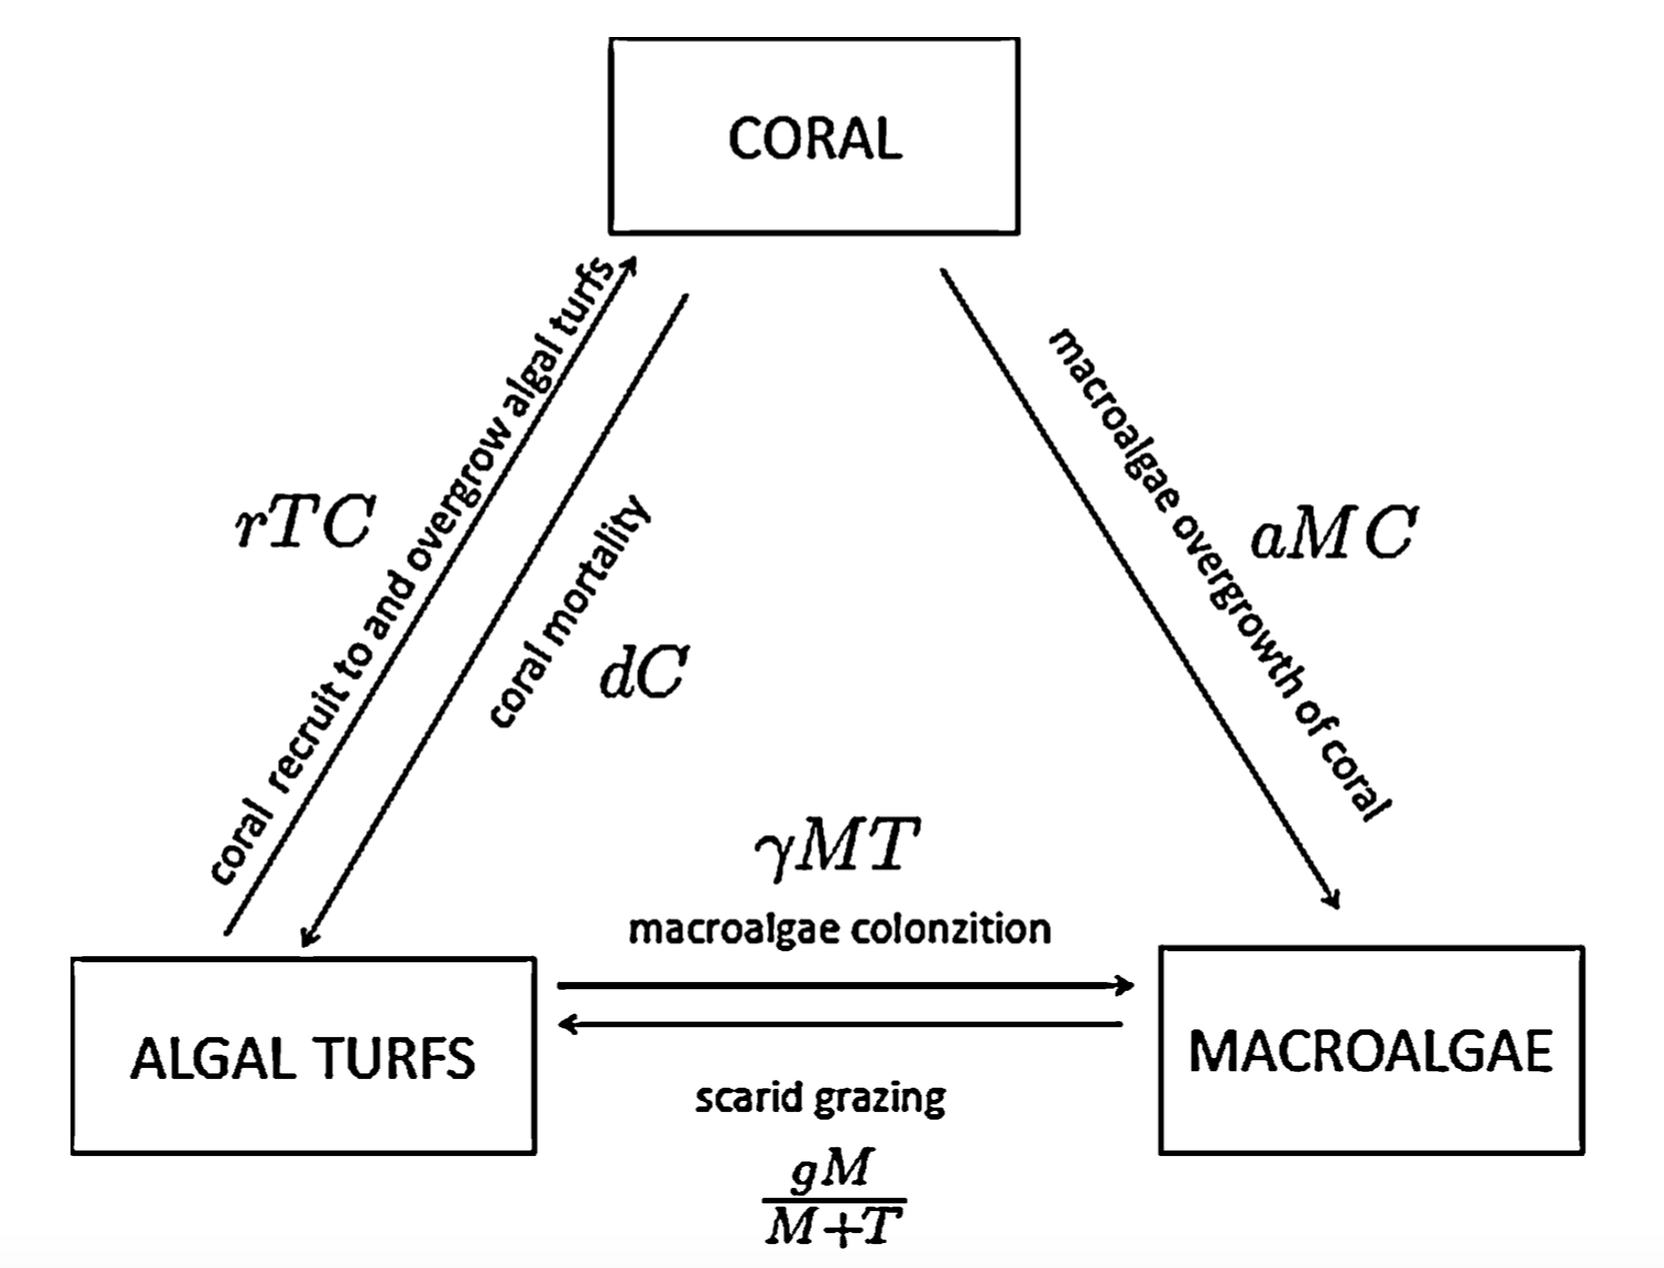
\includegraphics[scale=.175]{./coral-reef-triangle.png}
\end{frame}

\begin{frame}\frametitle{Coral Reef Dynamics}
The deterministic ordinary differential equation model:
$$\begin{cases}\begin{array}{rl}
\frac{dM}{dt}\hspace{-.8em}&=aMC - \frac{gM}{M+T} + \gamma M T, \\
\frac{dC}{dt}\hspace{-.8em}&=rTC - dC - aMC, \\
\frac{dT}{dt}\hspace{-.8em}&=\frac{gM}{M + T} - \gamma MT - rTC + dC. 
\end{array}\end{cases}$$ 

where 
\begin{itemize}\itemsep0pt
\item $r$ is the rate corals overgrow upon algal turfs\\
\item $d$ is the mortality rate of corals\\
\item $a$ is the rate that macroalgae overgrow upon corals\\
\item $\gamma$ is the rate that macroalgae spread over algal turfs\\
\item $g$ is the indiscriminate grazing rate of parrotfish.
\end{itemize}
\end{frame}

\begin{frame}\frametitle{Coral Reef Dynamics}

\hspace{1.57em}

\begin{itemize}
\item $\frac{dT}{dt}=-\frac{dM}{dt}-\frac{dC}{dt}$ implies $M+C+T$ is
  constant.
\item We assume that $M+C+T=1$.
\item This limits our scope to regions entirely covered by coral,
  macroalgae, and algal turf. 
\end{itemize}

Thus, we reduce our system to, 
$$\begin{cases}
\begin{array}{rl}
\frac{dM}{dt}&= aMC-\frac{gM}{1-C} + \gamma M - \gamma M^2 -\gamma M C,\\
\frac{dC}{dt}&=rC - rC^2 - rCM - dC - aMC.
\end{array} 
\end{cases}$$
\end{frame}


\begin{comment}\frametitle{Equilibria and Stability}
Equilibrium point

\end{comment}

\begin{frame}\frametitle{Equilibria and Stability}
To find equilibrium points analytically we first set the derivatives equal to zero to obtain the nullclines:
$$\begin{cases}
\begin{array}{rl}
0\hspace{-.8em}&=M(aC + \gamma-\gamma M-\gamma C) - \frac{gM}{1-C},\\
0\hspace{-.8em}&=C(r-Mr-Cr - d - aM).\\
\end{array}
\end{cases}$$
\end{frame}

\begin{frame}\frametitle{Equilibria and Stability}\begin{itemize}
\item $M'=0$ is satisfied when:\begin{itemize}\item $M=0$, or \item $aC + \gamma - \gamma M - \gamma C - \frac{gM}{1-C}=0$.\end{itemize}
\item $C'=0$ is satisfied when:\begin{itemize} \item$C=0$, or \item $r-Mr-Cr-d-aM=0$. \end{itemize}
\end{itemize}
\end{frame}

\begin{frame}\frametitle{Phase Plane} Our equilibrium points are located at the intersections of the nullclines:
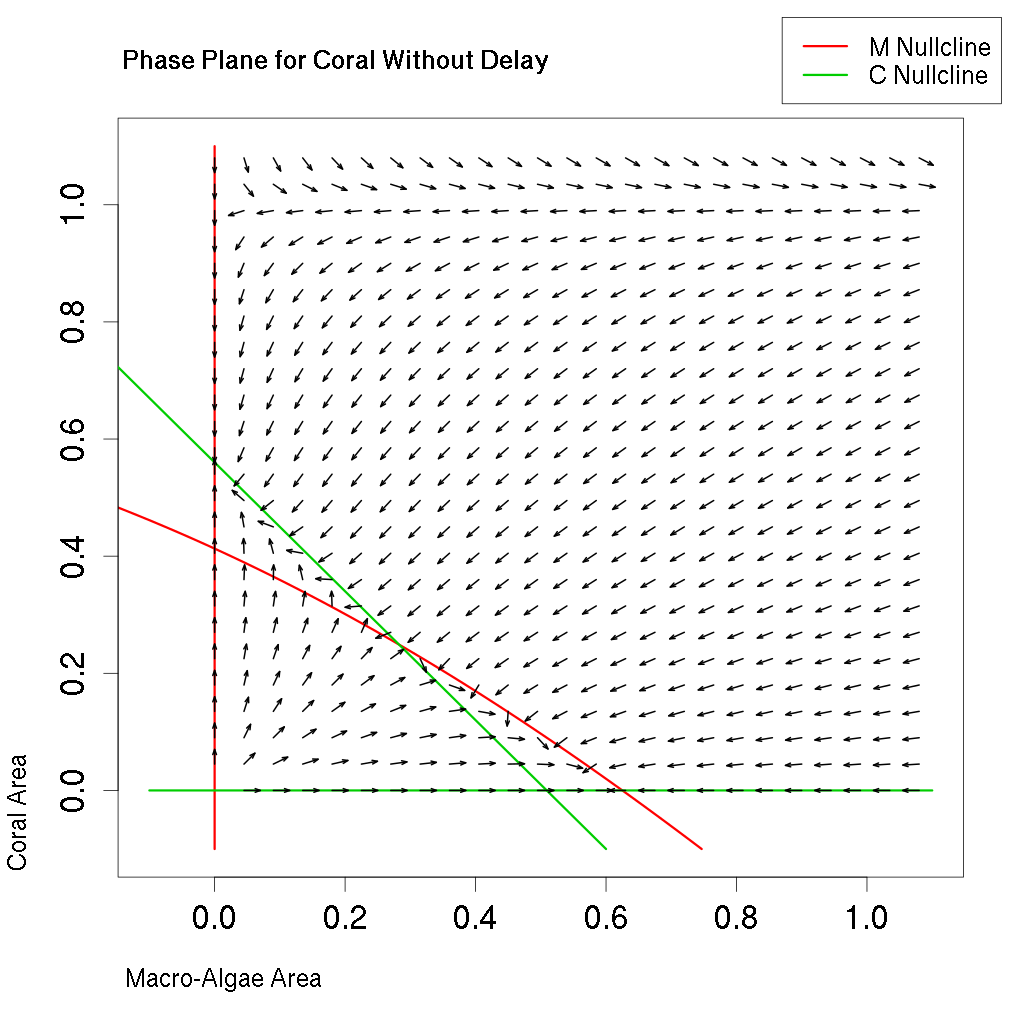
\includegraphics[scale=.22]{./nullclines.png}
\end{frame}

\begin{frame}
\frametitle{Time Delay in the Coral Ecosystem}
We can identify time delays in the coral ecosystem:
\begin{itemize}
\item the delay between overfishing of herbivores and growth of macroalgae.\\
\item the delay between the growth of algae and the effect of algae on coral (Jompa, 2003).\\
\item the delay between the grazing of macroalgae and growth of algal turf (Li et al., 2014).
\end{itemize} We focus on the third time delay.
\end{frame}

\begin{frame}\frametitle{Coral Reef Dynamics}
Delay Differential Equation Model:
$$\begin{cases}
\begin{array}{rl}
\frac{dM}{dt}\hspace{-.8em}&=aMC - \frac{gM(t-\tau)}{1-C(t-\tau)} + \gamma M (1-M-C),\\
\frac{dC}{dt}\hspace{-.8em}&=rC(1-M-C) - dC - aMC,\\
\end{array}
\end{cases}$$ where $\tau$ is our time delay.
\end{frame}

\begin{frame}
\frametitle{Equilibria and Stability}
There are three equilibrium points of interest: \begin{itemize}
\item $(0,0)$ (Unstable for all $\tau\geq0$)\\
\item $(1-\frac{g}{\gamma},0)$ (High Coral Cover)\\
\item $(0,1-\frac{d}{r})$ (High Algae Cover).
\end{itemize} Notice that time delay does not affect the equilibria.
\end{frame}

\begin{frame}\frametitle{Jacobian Matrices}
We linearize our delay model:{\small $\begin{bmatrix} M'\\C'\end{bmatrix}=J_1\begin{bmatrix} M\\C\end{bmatrix}+J_2\begin{bmatrix}M(t-\tau)\\C(t-\tau)\end{bmatrix}$ (call this eq'n 1), where $$J_1=\begin{bmatrix}\gamma-2\gamma M +(a-\gamma)C & (a-\gamma)M\\ -(a+r)C & r-d-(a+r)-2MC \end{bmatrix}, \text{ and}$$ $$J_2=\begin{bmatrix} \frac{-g}{1-C(t-\tau)} & \frac{-gM(t-\tau)}{(1-C(t-\tau))^2}\\ 0 & 0\end{bmatrix}.$$}
\end{frame}

\begin{comment}

\begin{frame}\frametitle{Putting Jacobians to Use}
{ Suppose $\begin{bmatrix} x\\y\end{bmatrix}=\overrightarrow{v_1}e^{\lambda t}$.}\\\vspace{2em} 
{ Differentiating, setting equal to 1, and doing algebra stuff, we get $(J_1+J_2e^{-\lambda t} -\lambda I)\overrightarrow{v_1}=0$.} 
\end{frame}
\end{comment}

\begin{frame}\frametitle{Putting Jacobians to Use}
Consider the Jacobians evaluated at the origin:$$J_1=\begin{bmatrix}
\gamma & 0\\
0 & r-d
\end{bmatrix}, \text{ and}$$ $$J_2=\begin{bmatrix}
-g & 0\\
0 & 0
\end{bmatrix}.$$ 
\end{frame}


\begin{frame}[c]\frametitle{Putting Jacobians to Use}
%Recall, $(J_1+J_2e^{-\lambda t} -\lambda I)\overrightarrow{v_1}=0$. \\\vspace{2em} Taking determinants, we find the characteristic polynomial of $(J_1+J_2e^{-\lambda t} -\lambda I)$ evaluated at $M=0$, $C=0$ to be 
The characteristic polynomial of $$(J_1+J_2e^{-\lambda t} -\lambda I),\text{ is}$$ $$(\lambda - r + d)(\lambda -\gamma + ge^{-\lambda\tau})=0$$. 
\end{frame}

\begin{frame}\frametitle{Get Them Eigenvalues}
Hence, \begin{itemize}{\itemsep .5in}\item $\lambda = r-d>0$ is an eigenvalue with positive real part\item Other eigenvalues satisfy $\lambda=\gamma-ge^{-\lambda\tau}$. \item For $\tau\geq0$, our system has two eigenvalues with positive real part. This implies our nondelay system is unstable at $(0,0)$. \end{itemize}\end{frame}

\begin{comment}
\begin{frame}\frametitle{Get Them Eigenvalues}
Now we consider postive $\tau$.
\begin{itemize}
\item Let $\lambda \tau=(\alpha+i\omega)\tau$.
\item Apply Euler's Formula: $\gamma-g(e^{-\lambda\tau})=\gamma-g(\cos(\lambda\tau)-i\sin(\lambda\tau))$.
\end{itemize}
\end{frame}\end{comment}

\begin{frame}
The time delay model fails to account for stochastic features of the ecosystem:
\begin{itemize}
\item grazing habits of parrotfish, and;
\item hurricanes.
\end{itemize}
\end{frame}

\begin{frame}
\frametitle{Stochastic Model}
To account for these stochastic feature we add noise!
$$\begin{cases}
\begin{array}{rl}
\frac{dM}{dt}\hspace{-.8em}&=aMC - \frac{gM(t-\tau)}{1-C(t-\tau)}+\gamma M T+\beta M(1-M)dW,\\
\frac{dC}{dt}\hspace{-.8em}&=rTC - dC - aMC.\\
\end{array}
\end{cases}$$
\end{frame}

\begin{frame}

\end{frame}

\section{Stochastic Differential Equations}

\begin{frame}
  \frametitle{SDEs!}

  A bunch of stuff goes here.

\end{frame}

\begin{frame}
  \frametitle{title}
  
\end{frame}

%%% Local Variables:
%%% mode: latex
%%% TeX-master: "Presentation1"
%%% End:


\section{Results}

\begin{frame}{Results}
  
  Revisiting the model
  $$\begin{cases}
    \begin{array}{rl}
      dM\hspace{-.8em}&=[aMC - \frac{gM(t-\tau)}{1-C(t-\tau)} + \gamma M (1-M-C)]dt+\beta M(1-M)dW,\\
      dC\hspace{-.8em}&=[rC(1-M-C) - dC - aMC]dt.\\
    \end{array}
    \end{cases}$$\\
  We are interested in the effects of:
  \begin{itemize}
  \item $\theta$ (the initial condition)\\
  \item $\beta$\\
  \item $\tau$\\
  \item $g$\\
  \end{itemize}
  
  

\end{frame}

\begin{frame}{Theta}
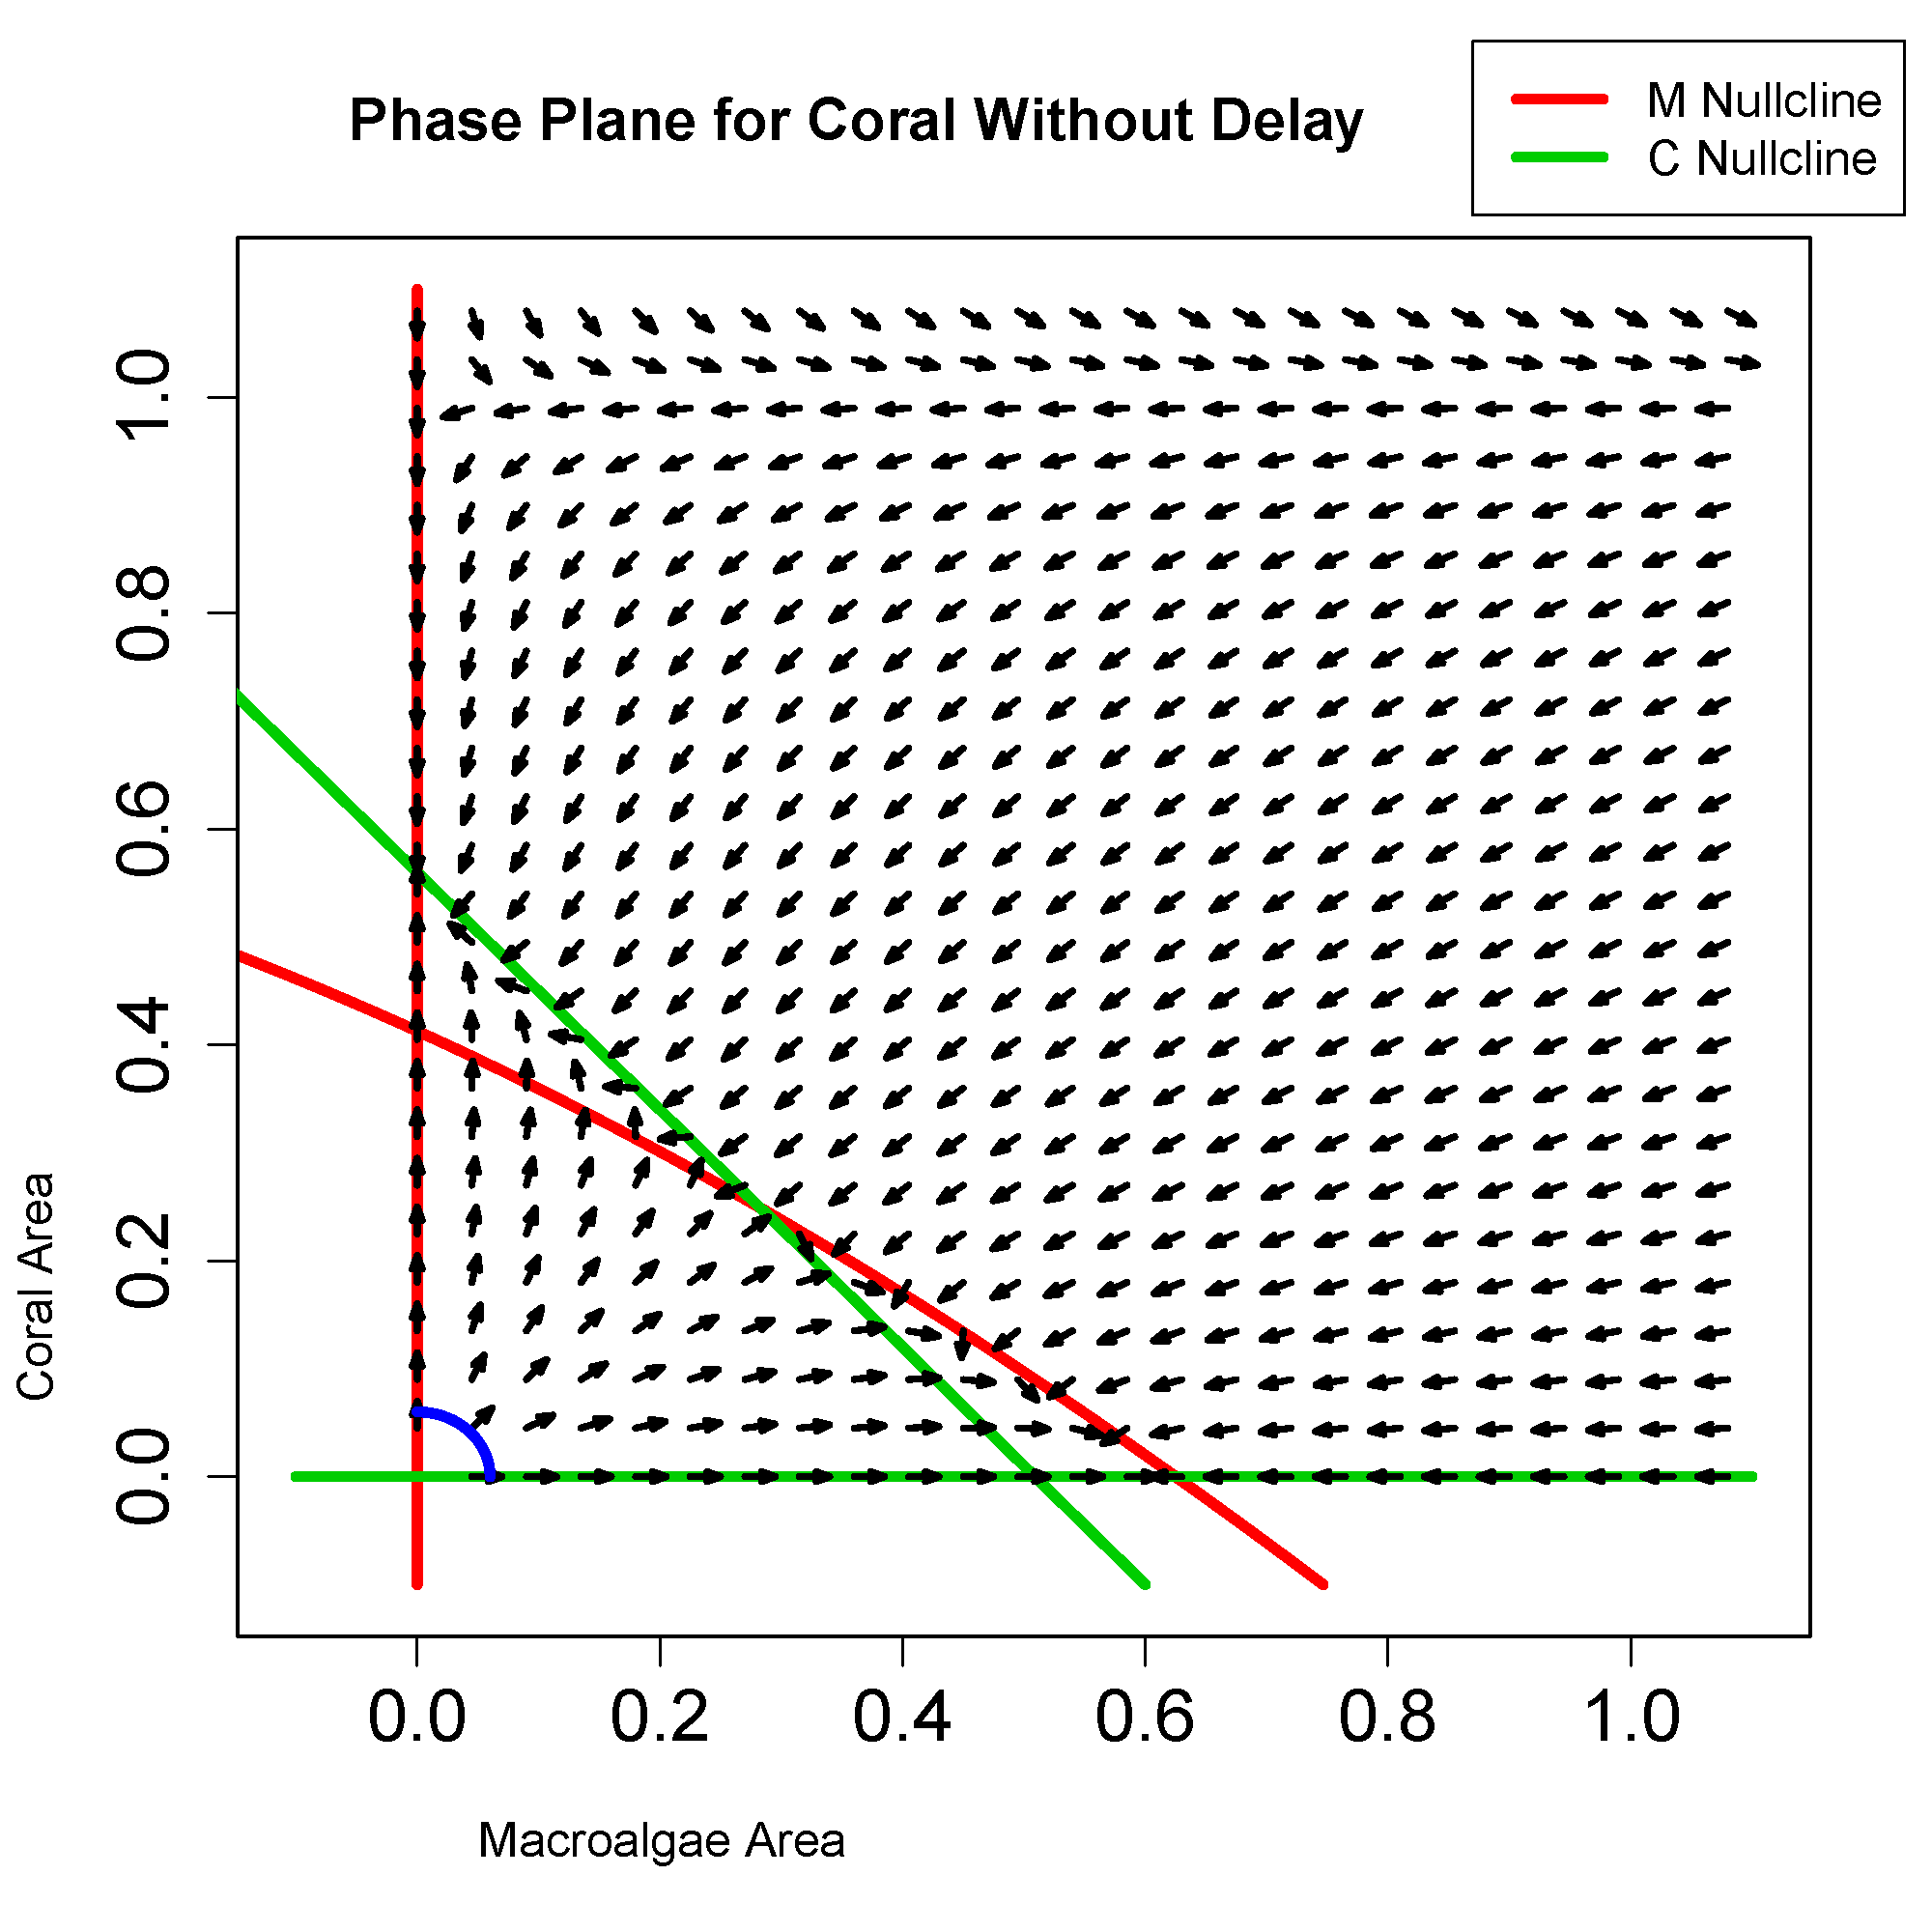
\includegraphics[scale=.325]{nullclinesarc.png}

\end{frame}

\begin{frame}{The Simulation}
We sampled the following values:
\begin{itemize}
\item $\theta$ = $\frac{\pi}{80}$ to $\frac{39\pi}{80}$ by $\frac{\pi}{80}$\\
\item $\beta$ = 0 to 1 by 0.05\\
\item $\tau$ = 0.5 to 1 by 0.05\\
\item $g$ = 0.2 to 0.8 by 0.1\\
\end{itemize}
\end{frame}

% %\begin{frame}\frametitle{At First Glance}
% %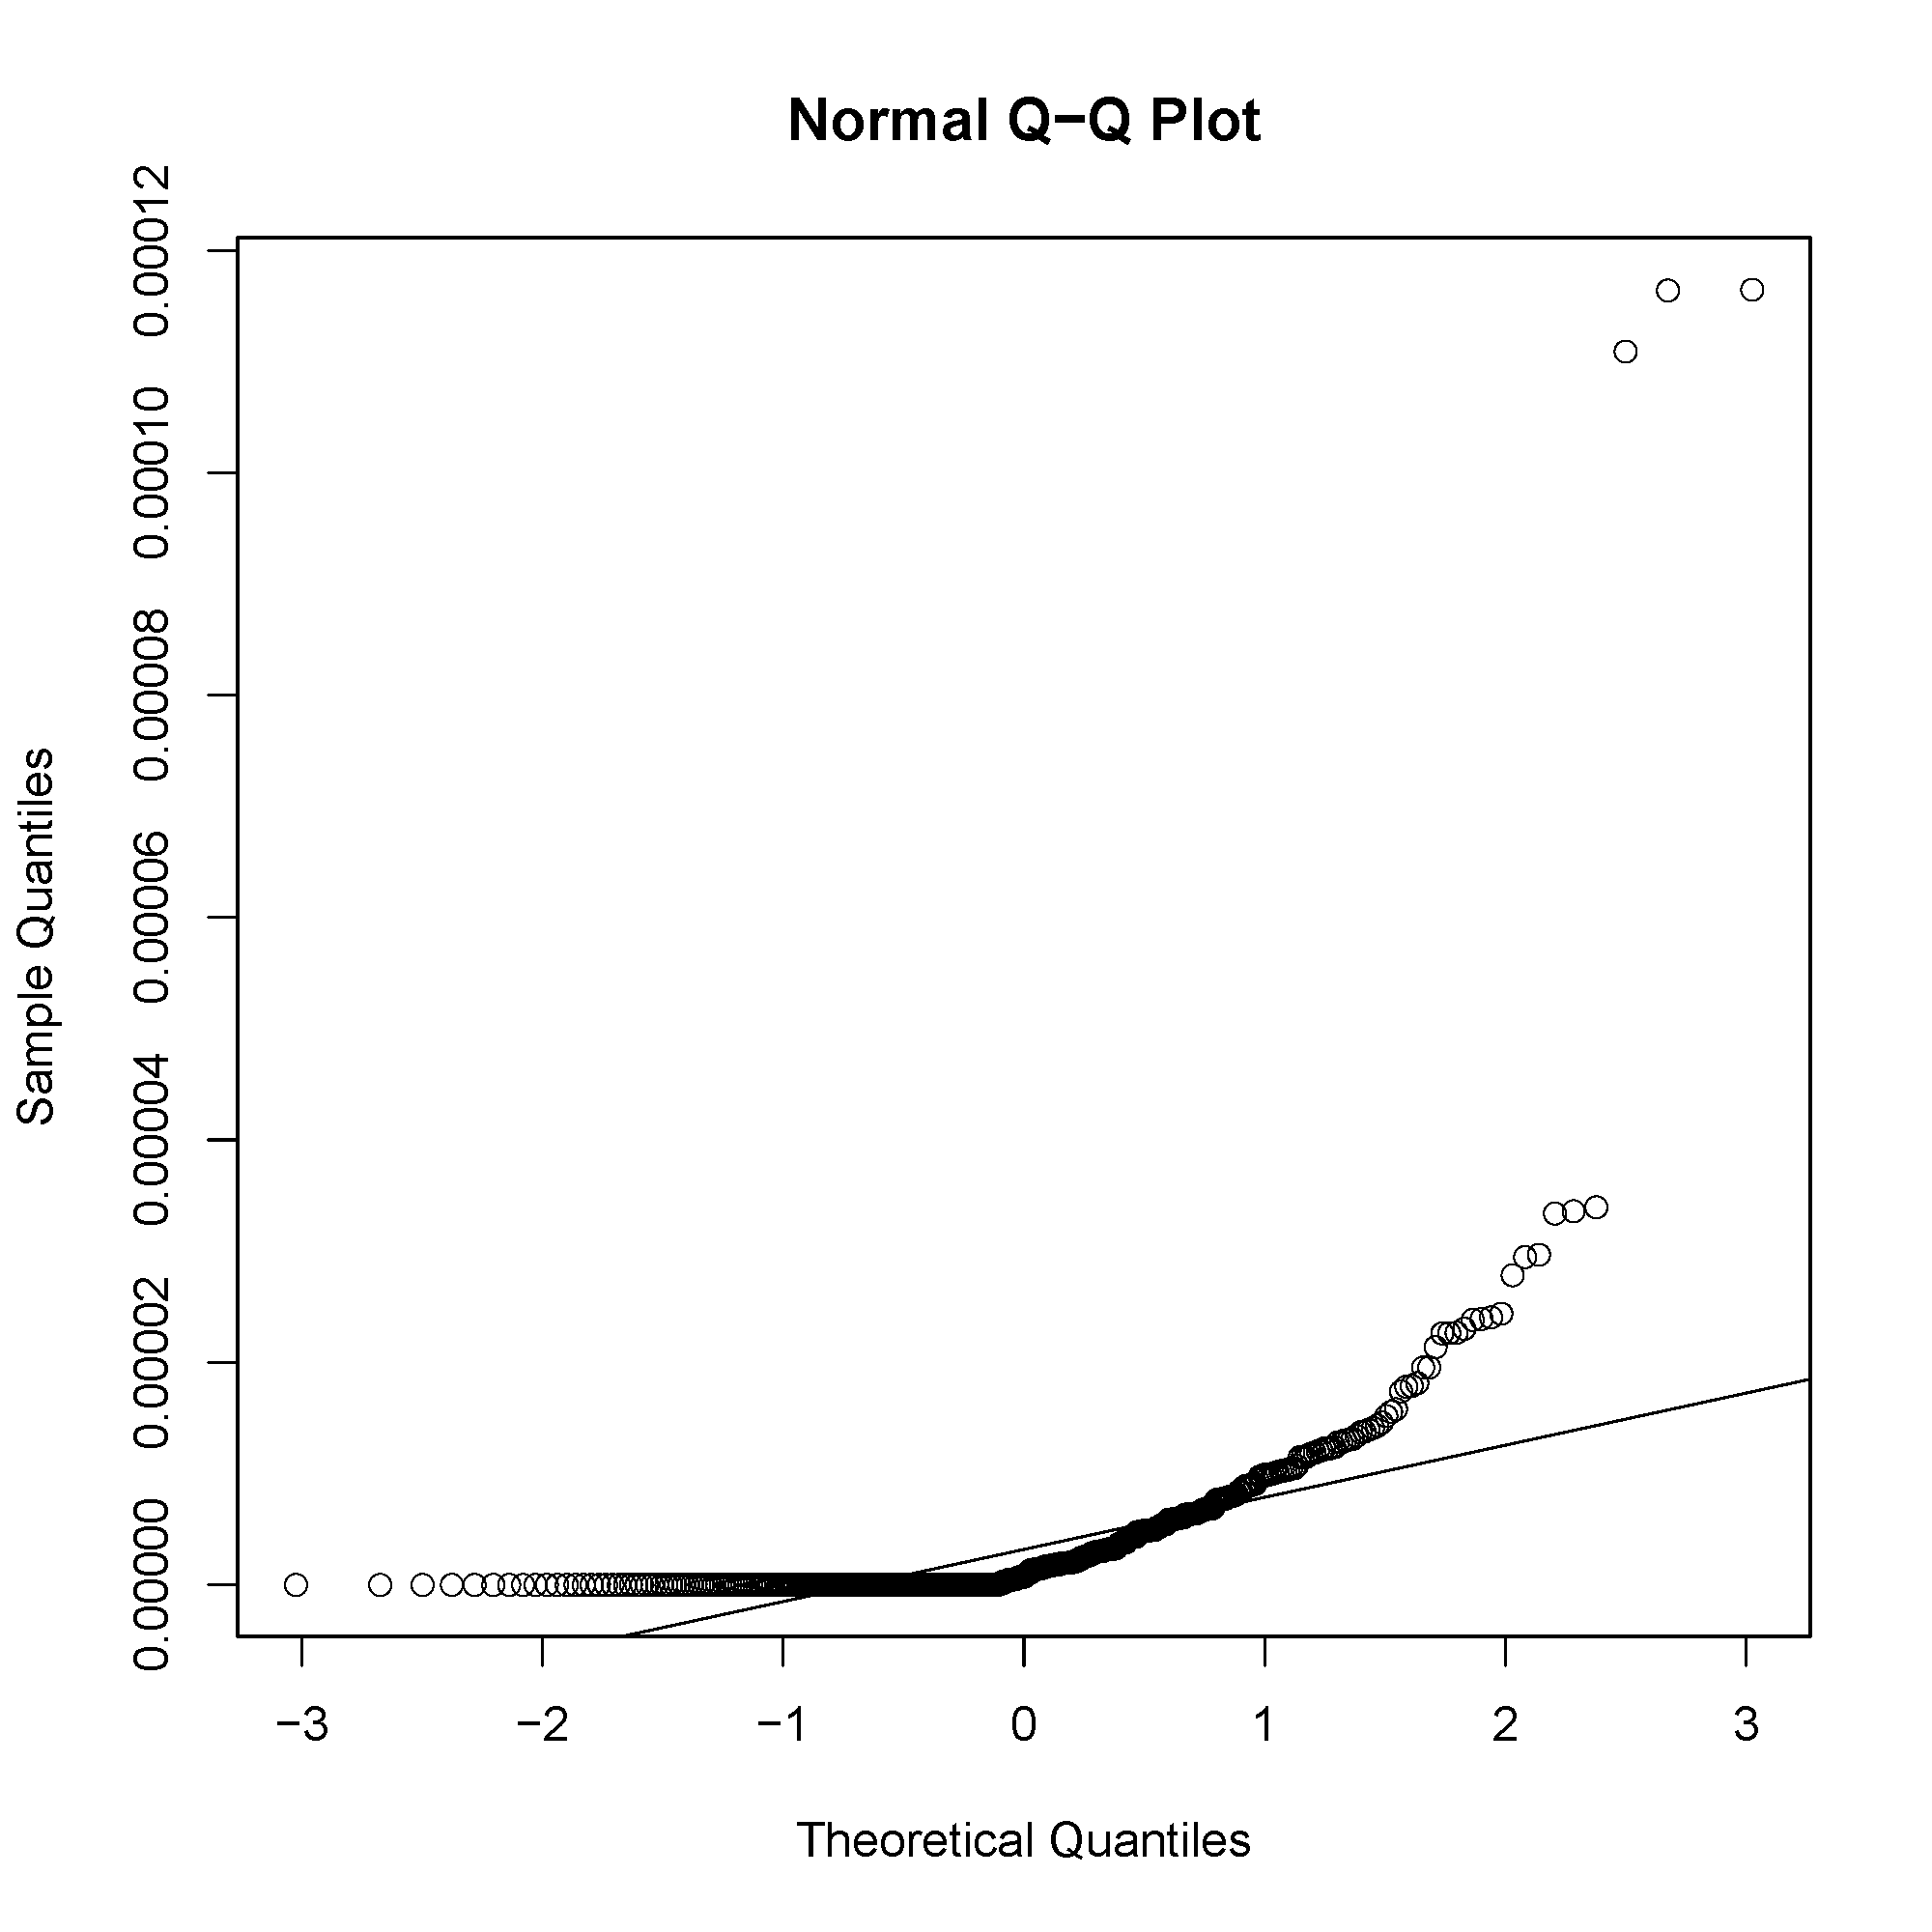
\includegraphics[scale=.325]{qqplot_lgcoral.png}
% %\end{frame}

\begin{frame}
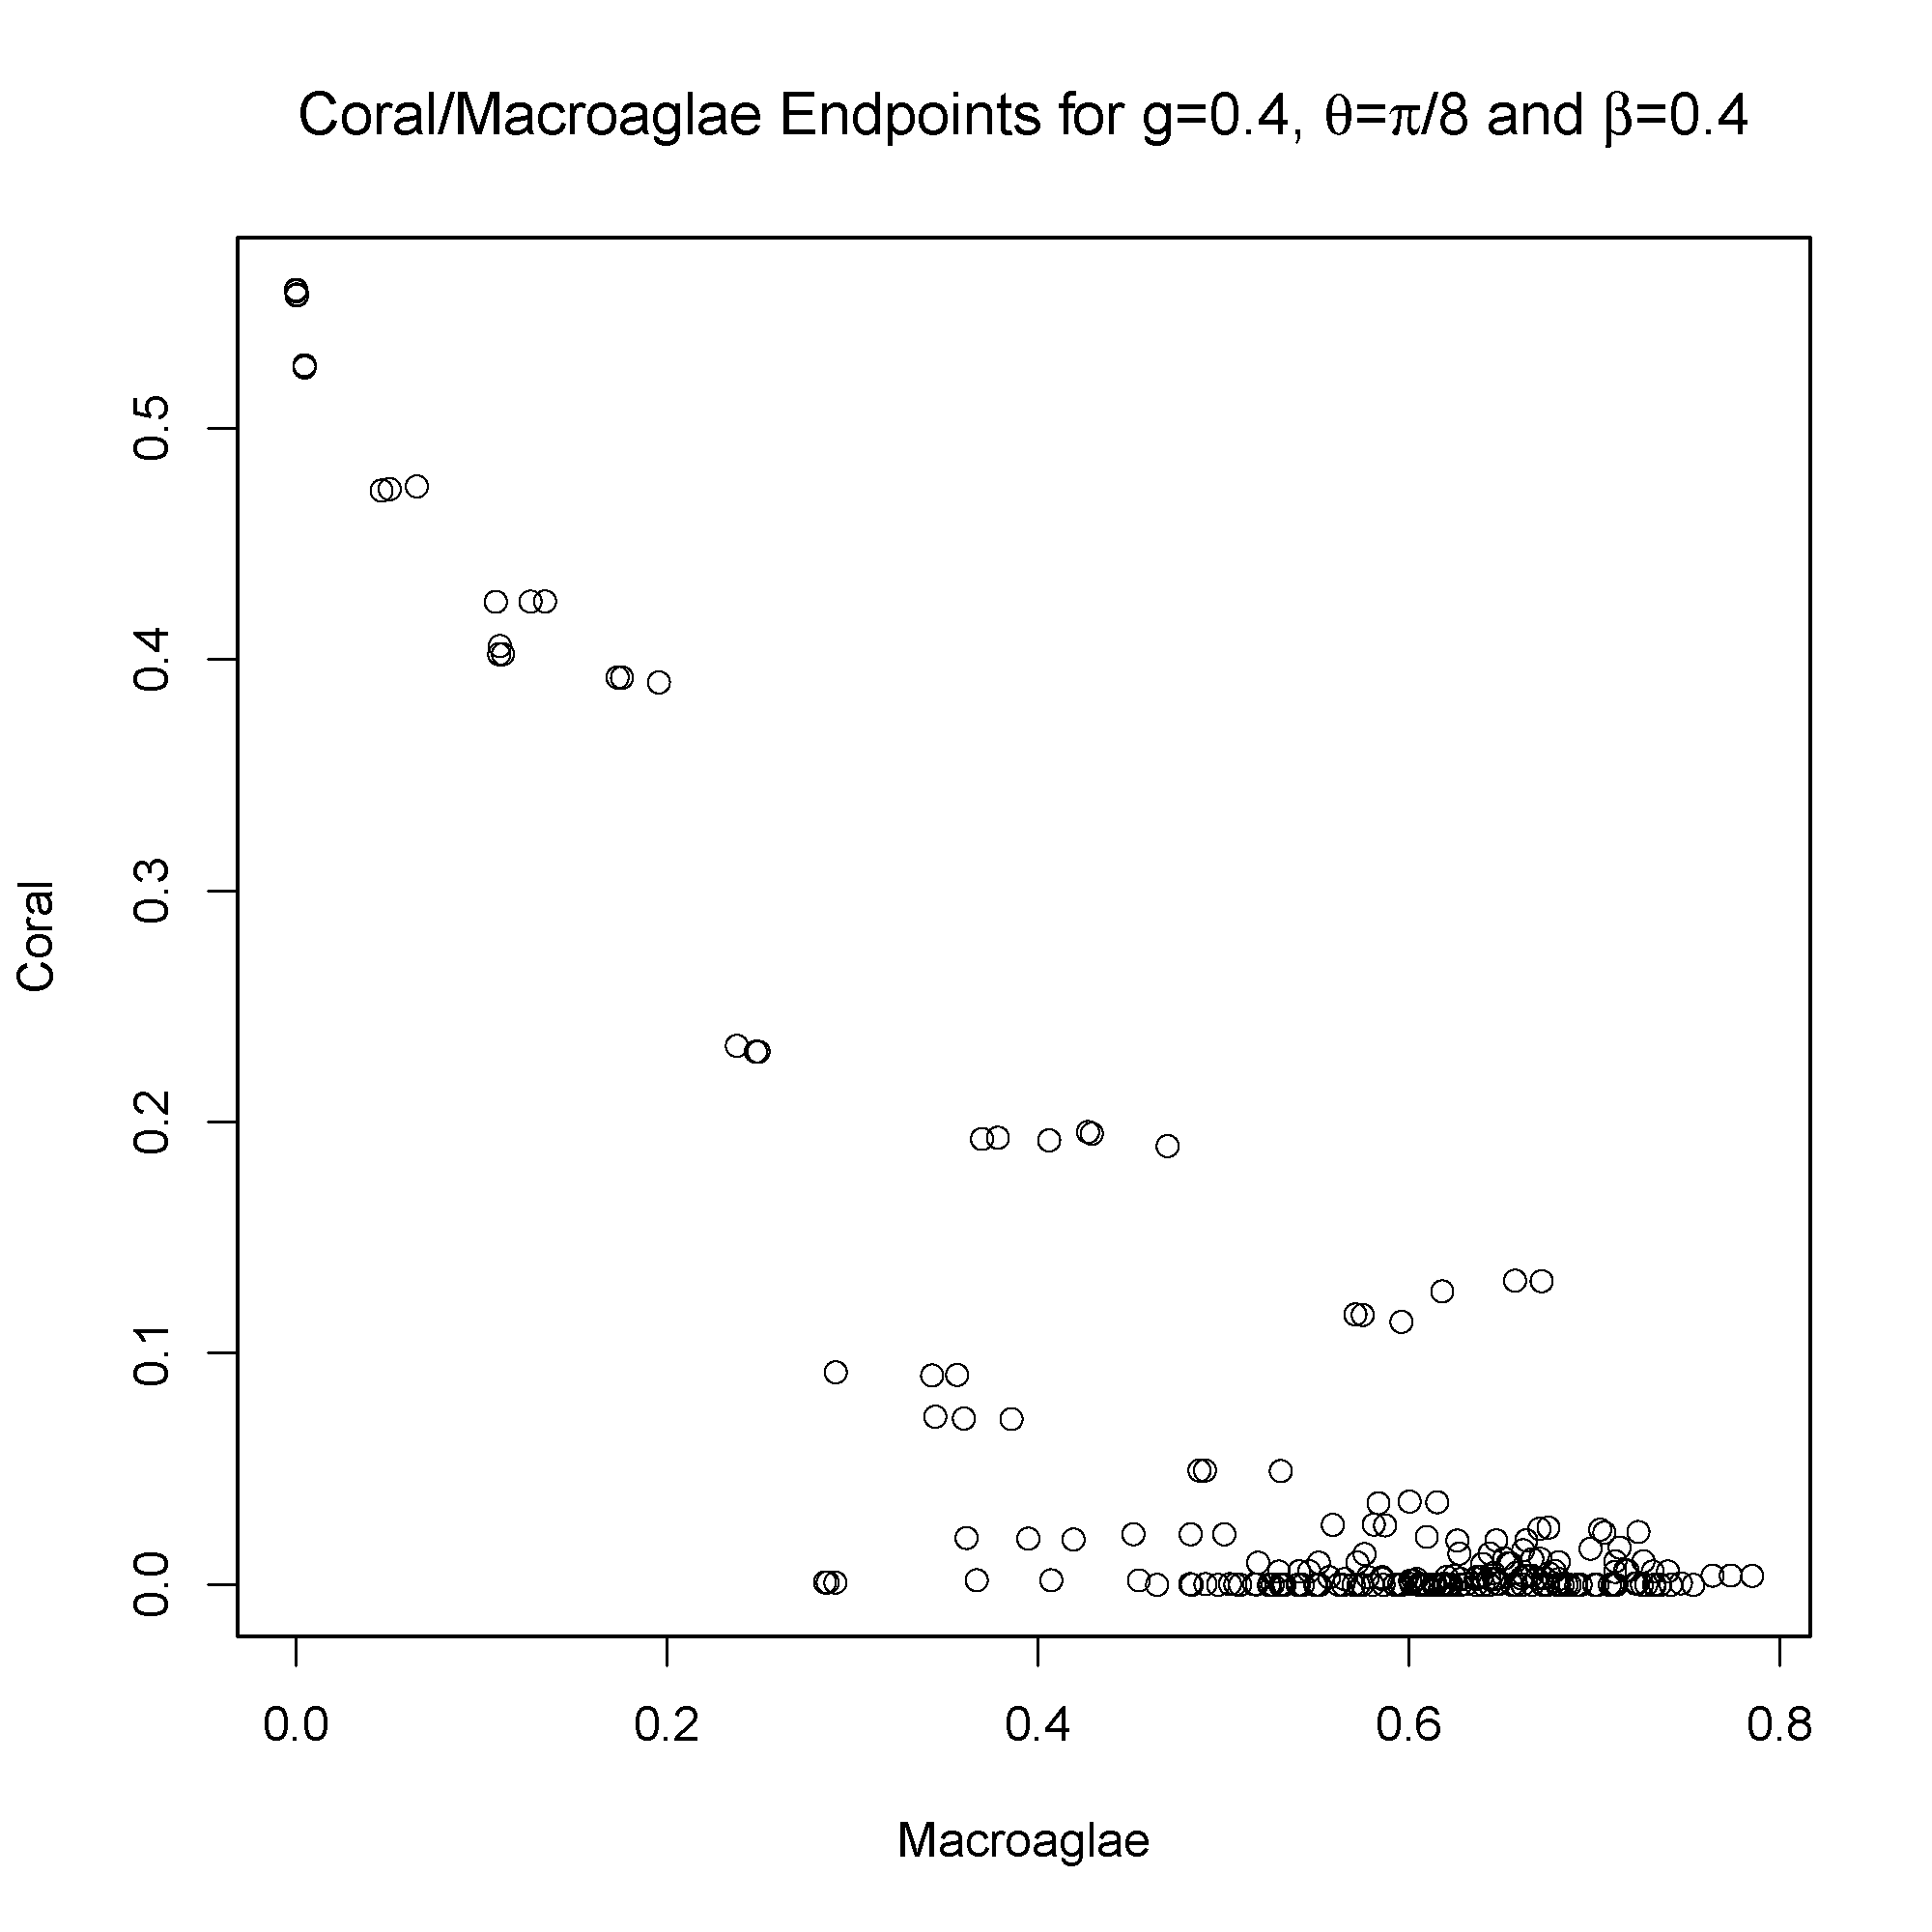
\includegraphics[scale=.325]{scatter_lgcoral_gpt4_betapt4_theta10.png}
\end{frame}

\begin{frame}{Initial Conditions}
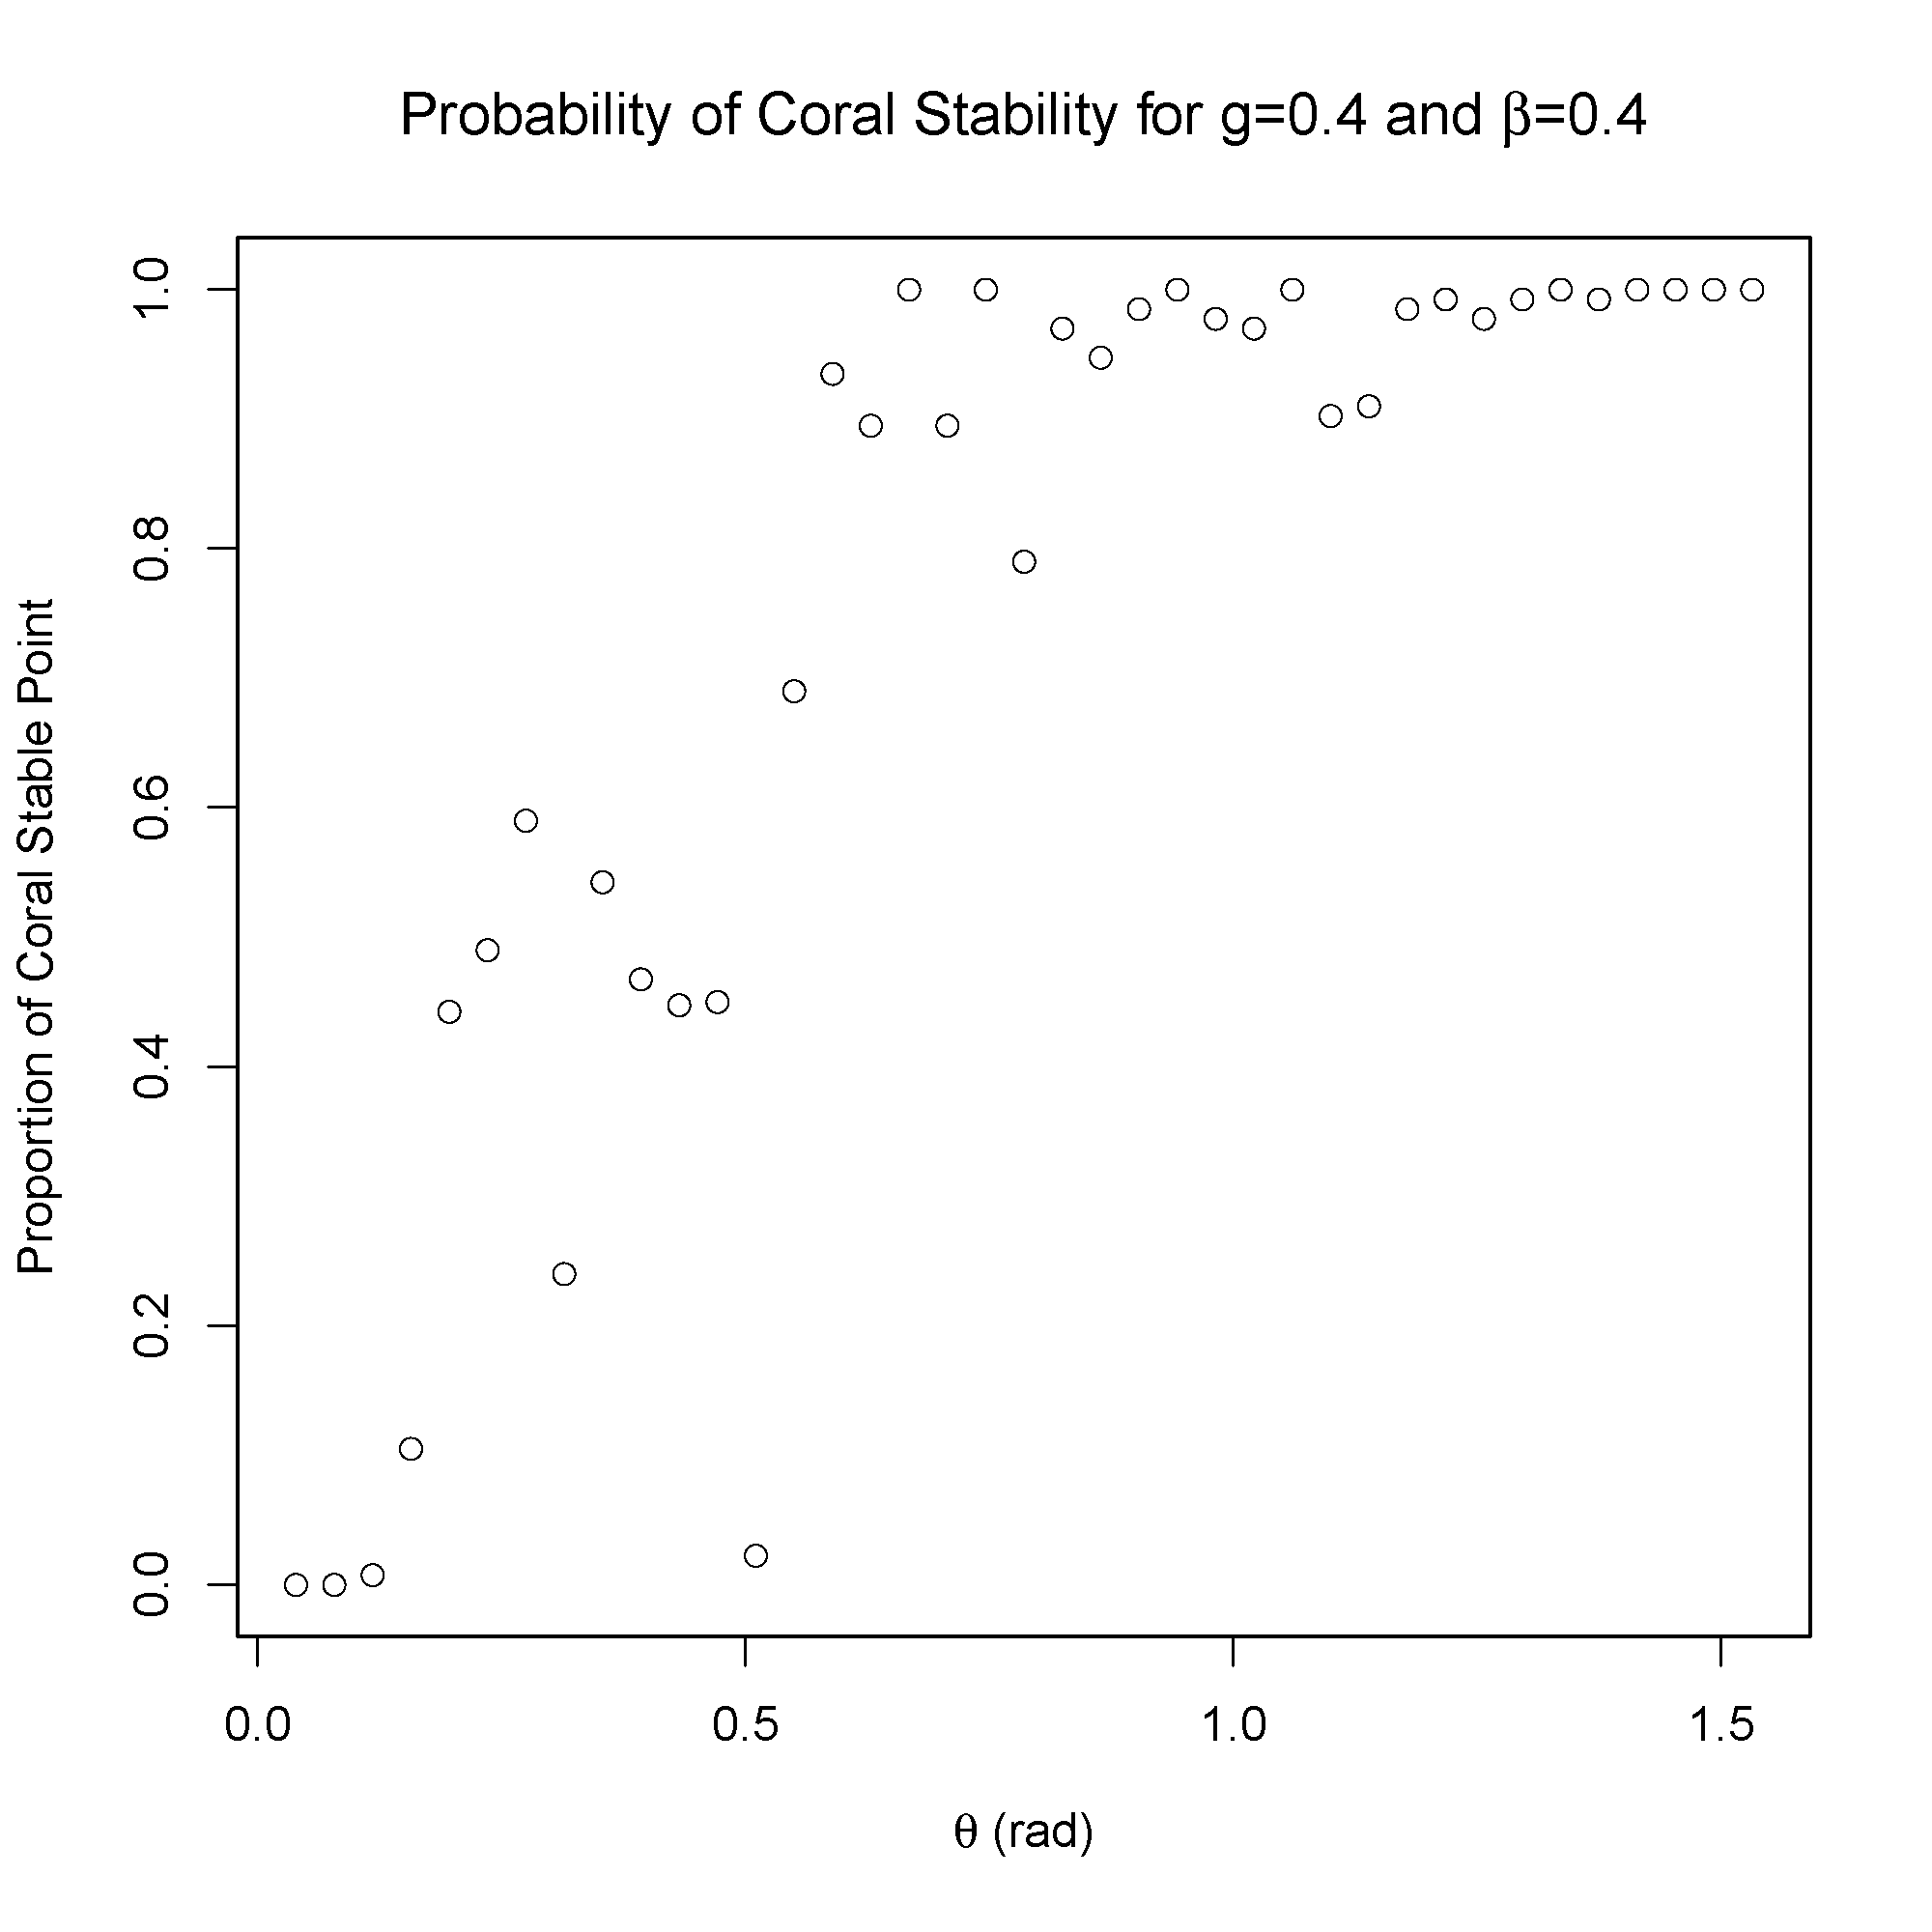
\includegraphics[scale=.325]{scatter_gpt4_betapt4.png}
\end{frame}

\begin{frame}{The Three Models}
Based on the plot, we will try the following three models
\begin{itemize}
\item Binomial Logit\\
Fits the model $logit(p)=a+b\theta$ where $logit(p)=log(\frac{p}{1-p})$\\
\item Poisson Log\\
Fits the model $log(n)=a+b\theta$\\
\item Ordinary Least Squares (OLS)\\
Fits the model $p=a+b\theta$\\
\end{itemize}
\end{frame}




\begin{frame}\frametitle{The Binomial Logit Model}
{\fontsize{8}{3} \color{RBlue} \verbatiminput{theta_logit_summary.txt}}

Conducting a goodness of fit test: \\
$P(\chi^{2}_{1}>10485-2171)<0.0001$\\

\end{frame}

\begin{frame}\frametitle{The Poisson Log Model}
{\fontsize{8}{3} \color{RBlue} \verbatiminput{theta_log_summary.txt}}

Conducting a goodness of fit test: \\
$P(\chi^{2}_{1}>3714.9-1970.4)<0.0001$\\

\end{frame}

%\begin{frame}\frametitle{Problematic Poisson}
%From the summary statistics, there is a problem with overdispersion.\\
%\\
%$\frac{G^2}{df}\approx1$\\
%$\frac{2006.7}{37}\approx54.2$\\
%\\
%Therefore, we fit a negative binomial model.\\
%\end{frame}

%\begin{frame}\frametitle{The Negative Binomial}

%\end{frame}

\begin{frame}\frametitle{Problematic Poisson}
There may be a problem with the model.
In the data, there is an overabundance of zeros.
Therefore, we fit a zero-inflated Poisson model (ZIP).
{\fontsize{8}{3} \color{RBlue} \verbatiminput{theta_zeros.txt}}
\end{frame}

\begin{frame}\frametitle{The ZIP Model}
{\fontsize{8}{3} \color{RBlue} \verbatiminput{theta_log_zip_summary.txt}}
\end{frame}

\begin{frame}\frametitle{The OLS Model}
{\fontsize{8}{3} \color{RBlue} \verbatiminput{theta_ols_summary.txt}}

Conducting a goodness of fit test: \\
$P(\chi^{2}_{1}>4.5824-1.4317)\approx0.07589$\\

\end{frame}

\begin{frame}\frametitle{Comparing the Models}
Our three models are \\
\begin{itemize}
\item Binomial Logit $p=\frac{e^{-2.48378+6.01631\theta}}{1+e^{-2.48378+6.01631\theta}}$\\
\item Poisson Log $n=e^{4.89295+0.90423\theta}$\\
\item OLS $p=0.22856+0.64310\theta$\\
\end{itemize}
How do we determine which model is the most appropriate?\\
\end{frame}

\begin{frame}{Binomial Logit, Poisson Log, or OLS}
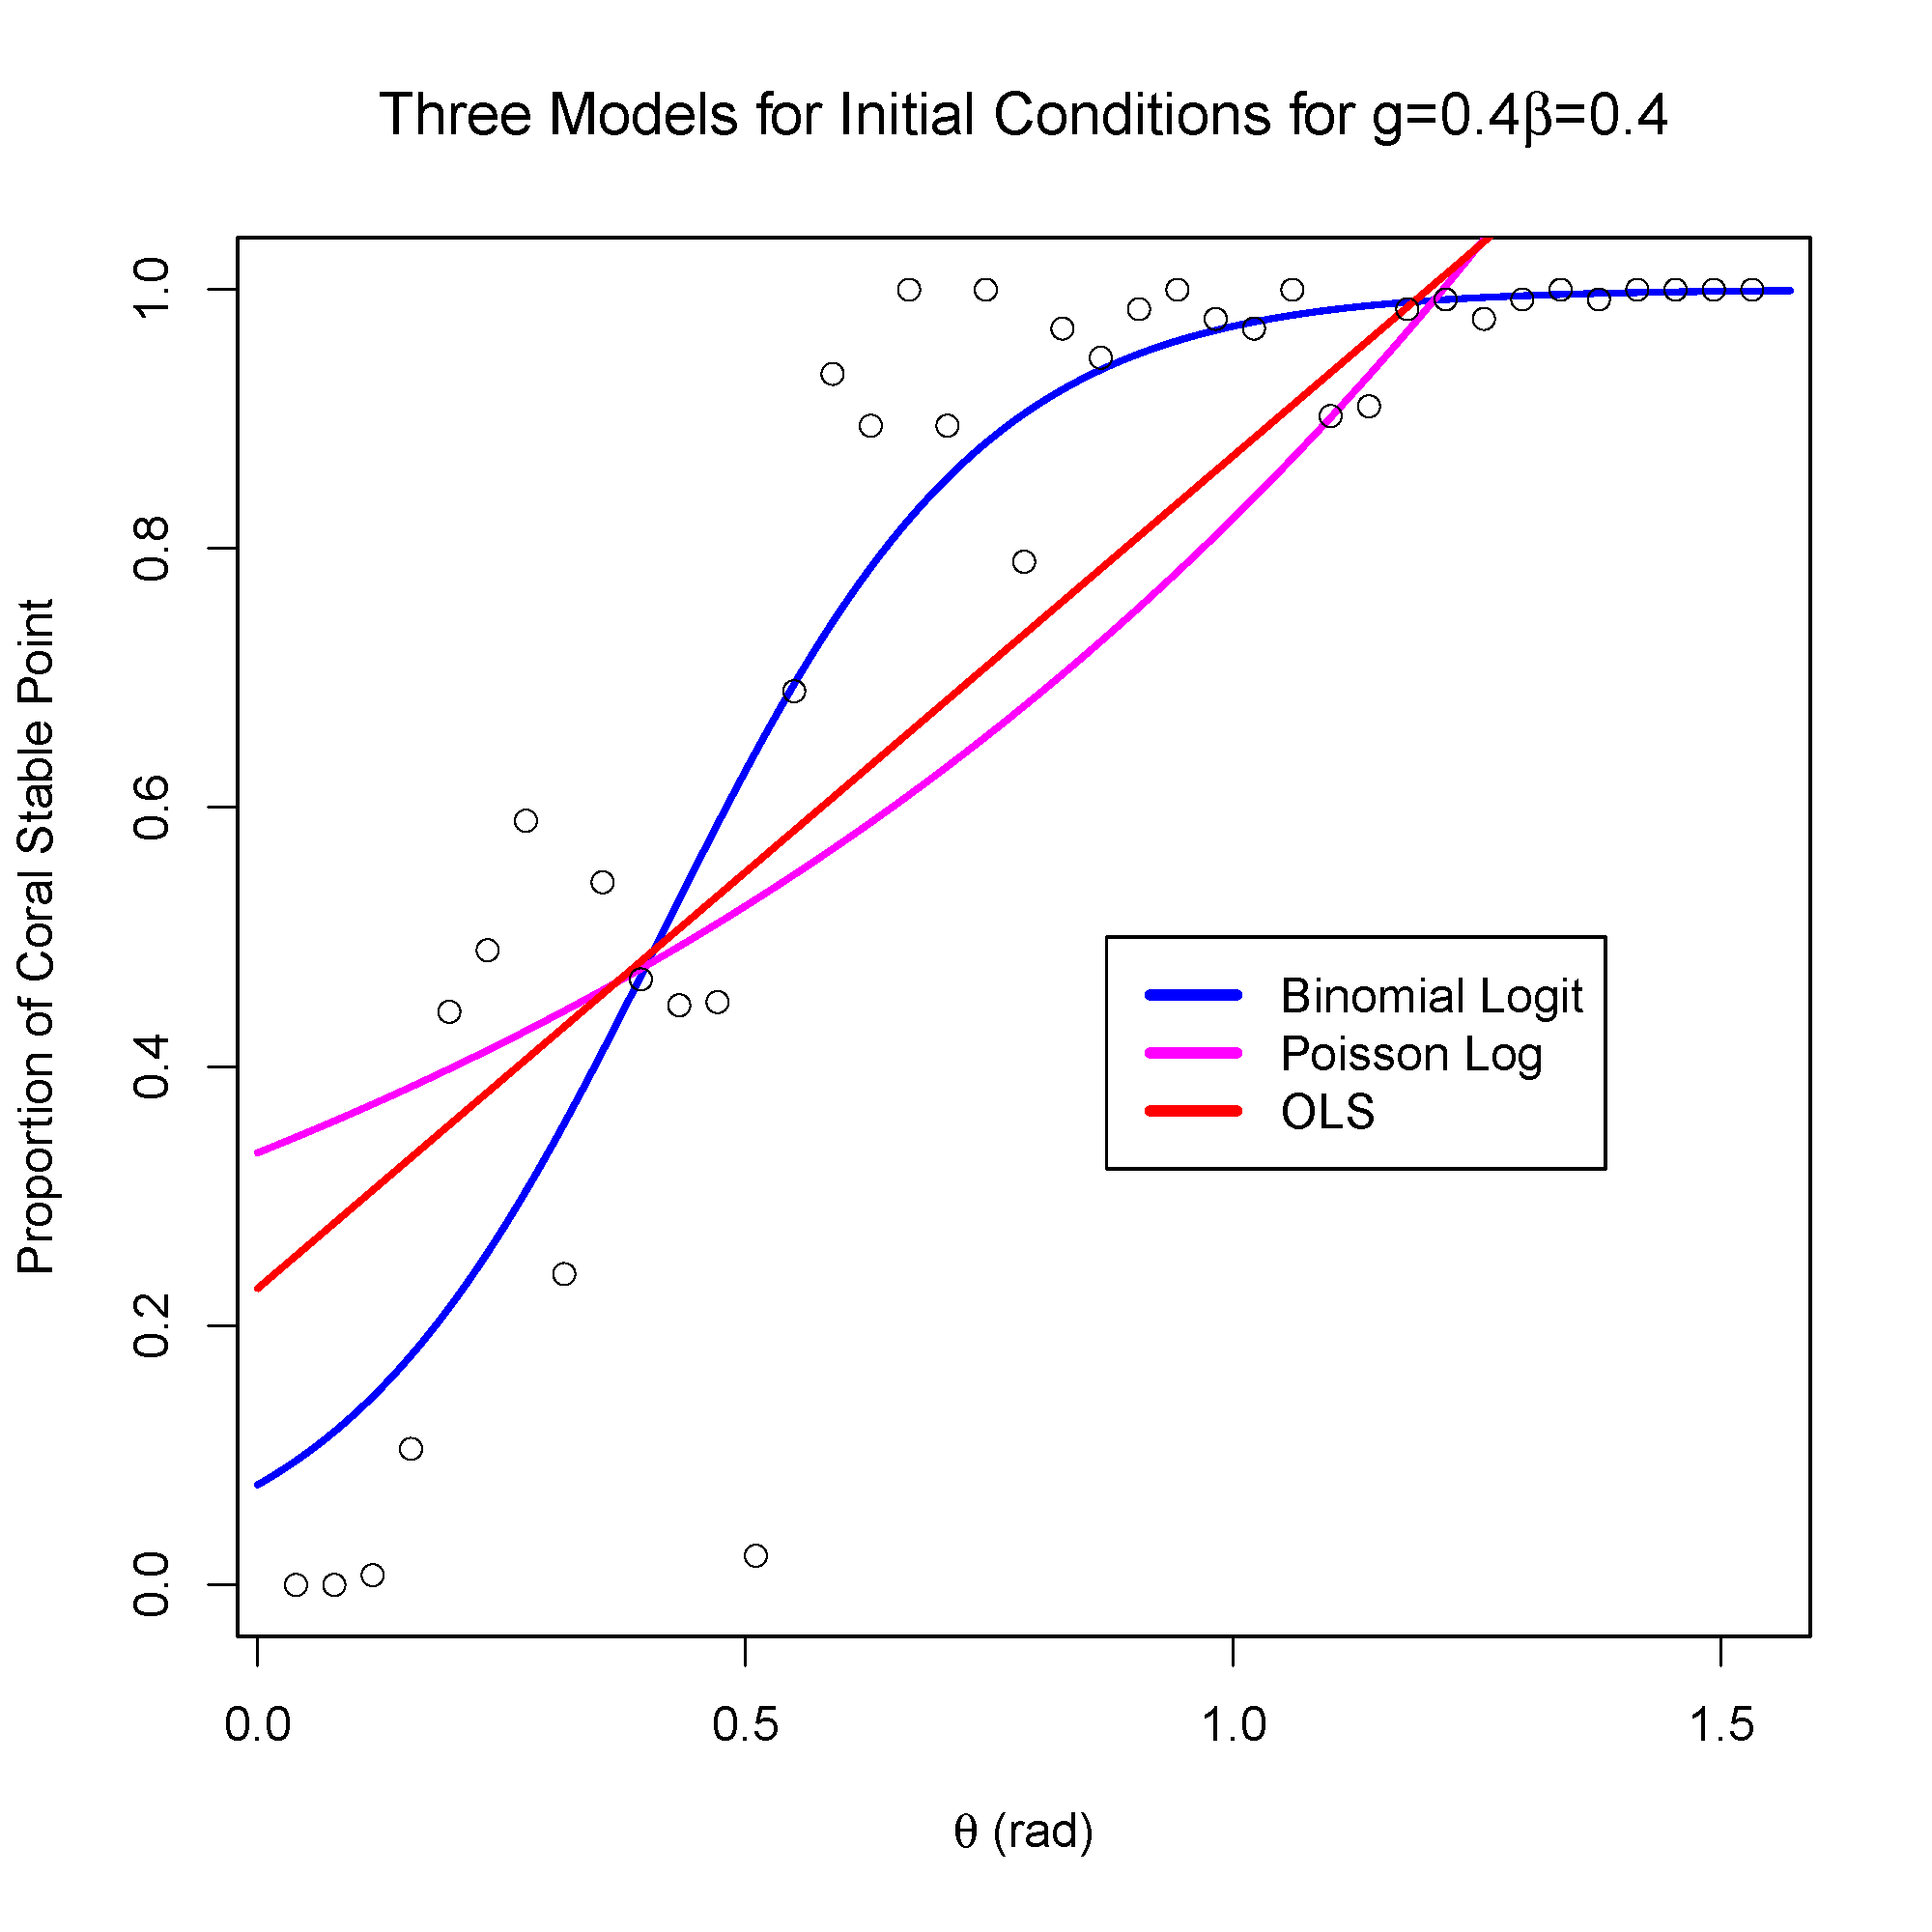
\includegraphics[scale=.325]{theta_threemodels.png}
\end{frame}

\begin{frame}\frametitle{The Whole Picture}
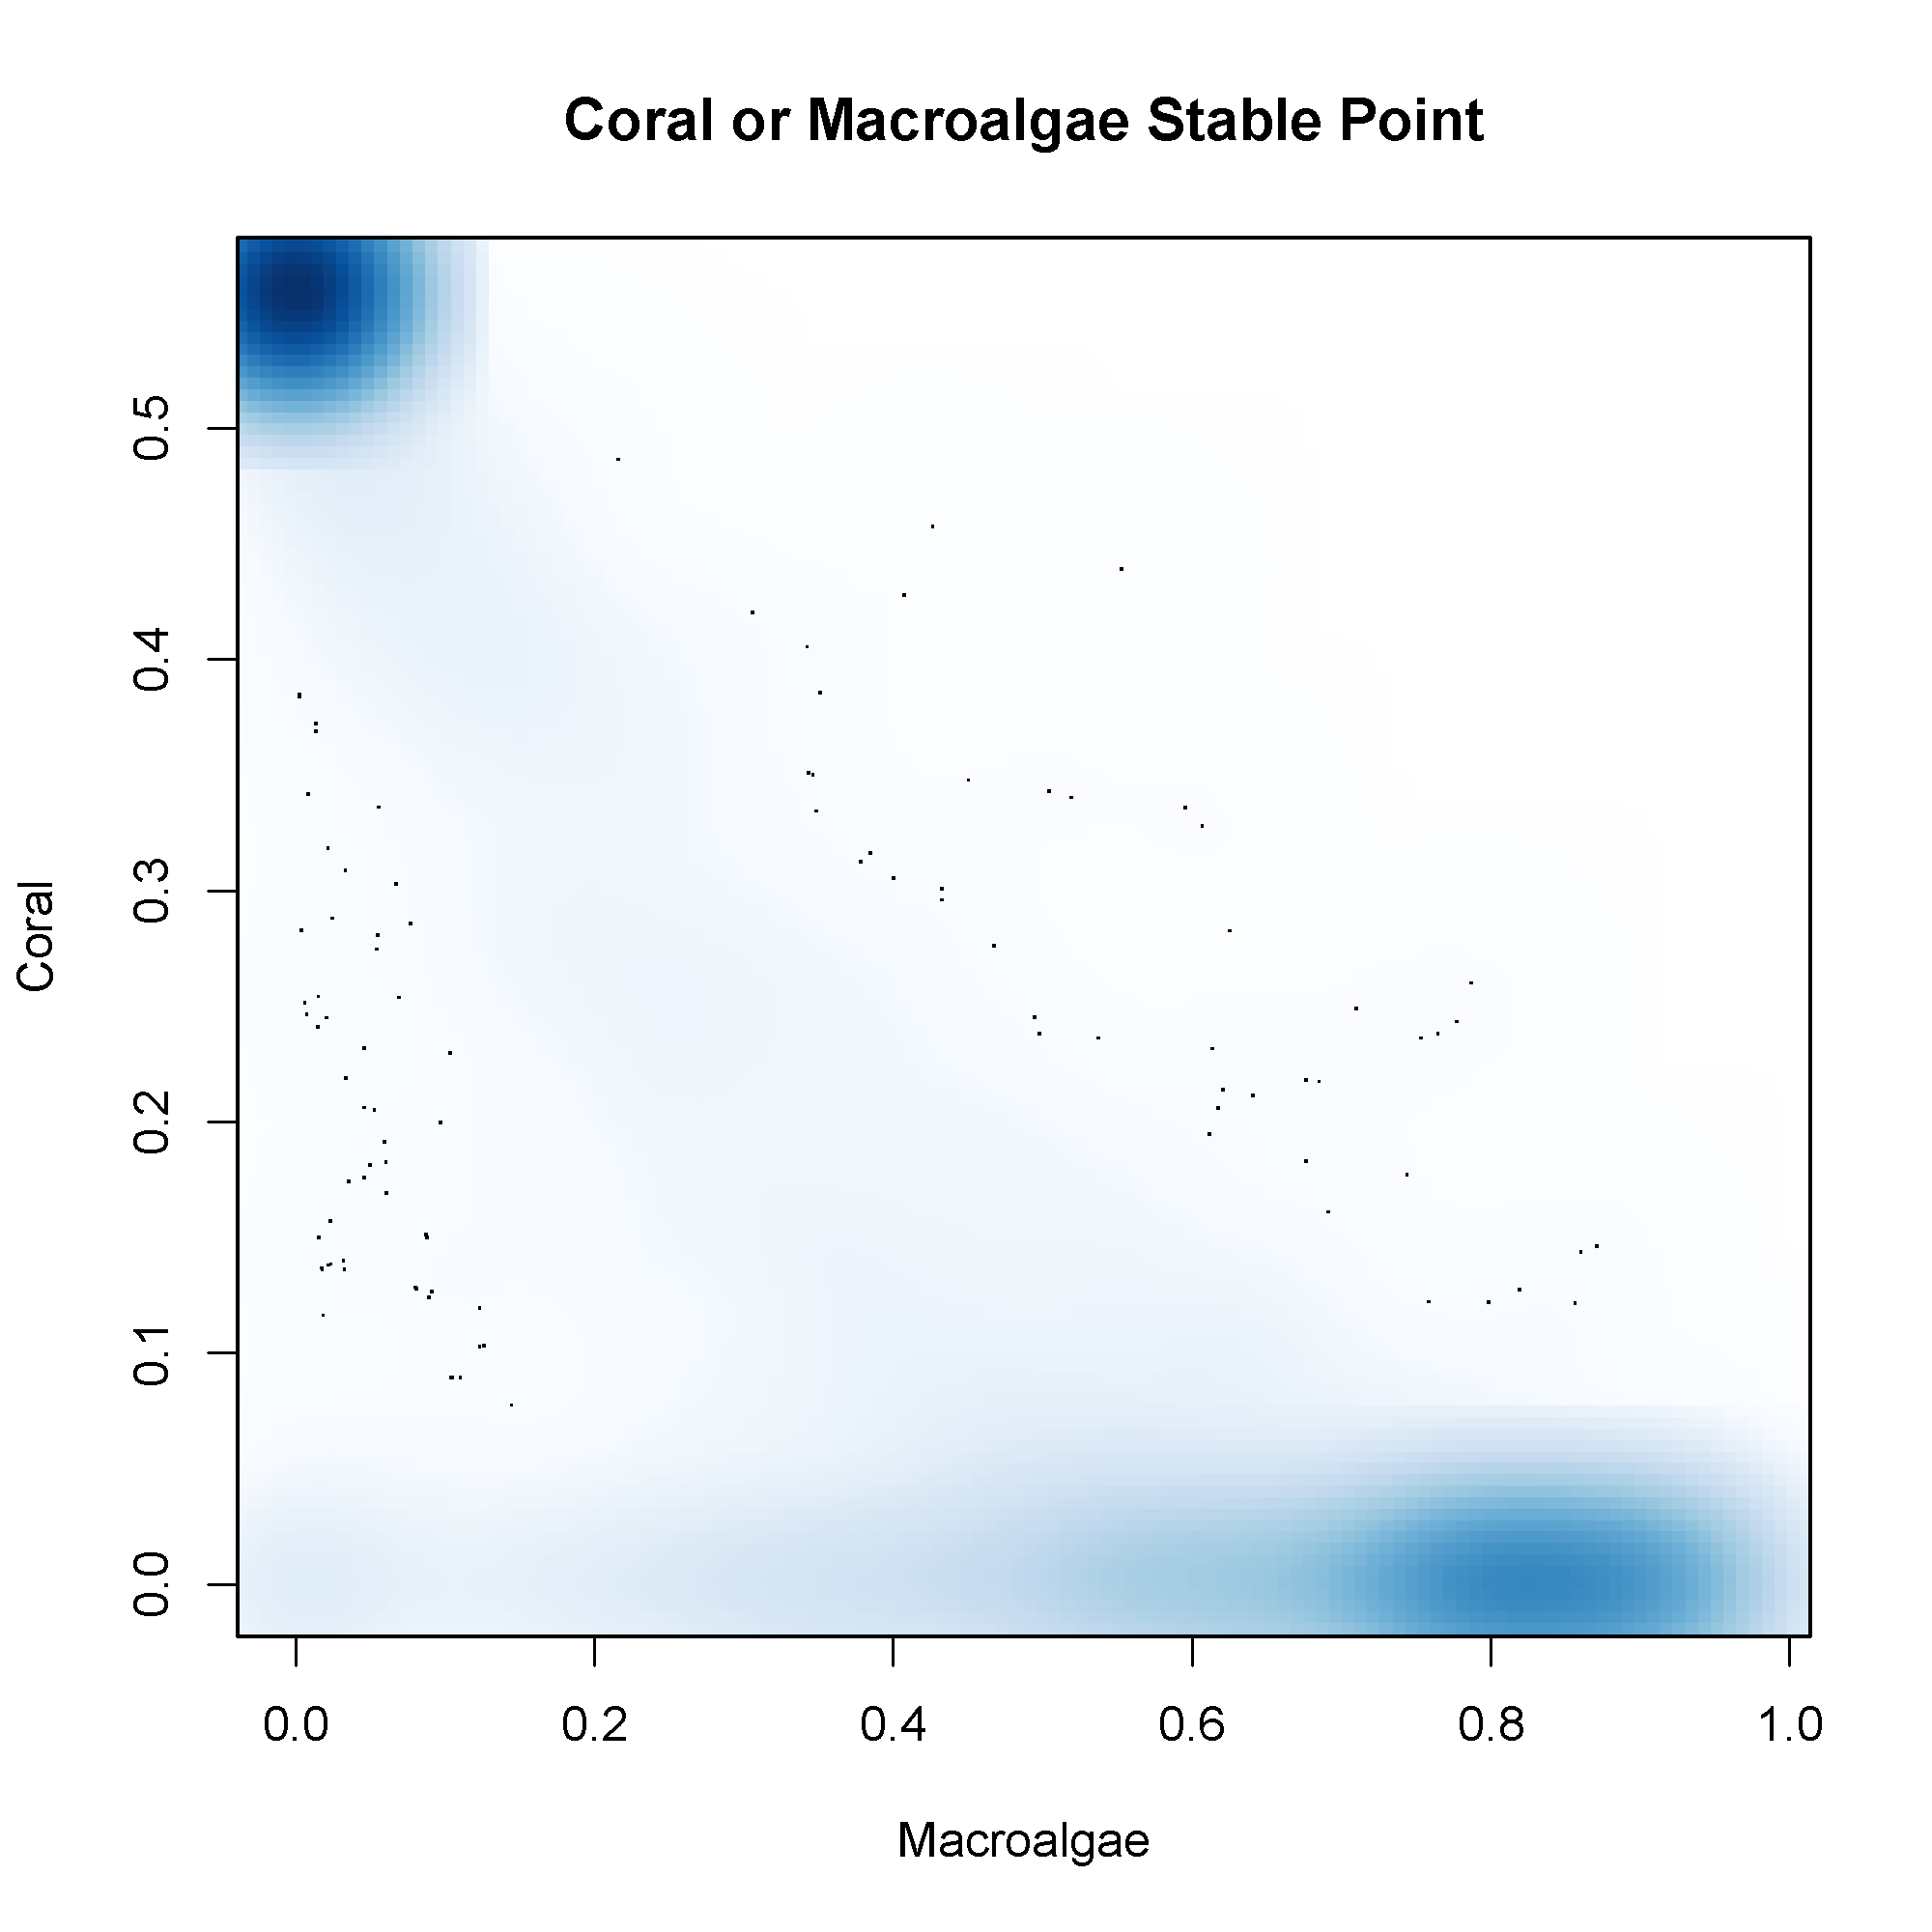
\includegraphics[scale=.325]{unifiedplot.png}
\end{frame}

\begin{frame}\frametitle{The Binomial Logit}
{\fontsize{8}{3} \color{RBlue} \verbatiminput{all_logit_summary.txt}}
\end{frame}

\begin{frame}\frametitle{Interpreting the Results}
Keeping theta and beta constant, an increase in g of:
\begin{itemize}
\item 0.01 has an odds ratio of coral survival of 3.21\\
\item 0.1 has an odds ratio of coral survival of 116413.1
\end{itemize}
\end{frame}

%%% Local Variables:
%%% mode: latex
%%% TeX-master: "Presentation2"
%%% End:

\section{Conclusions}

\begin{frame}
  \frametitle{Conclusions}

  A bunch of stuff goes here.

\end{frame}

\begin{frame}
  \frametitle{title}
  
\end{frame}

\begin{frame}
  \frametitle{Bibliography}
  
\end{frame}

\begin{frame}
  \frametitle{Acknowledgments}
  
  We would like to thank the following for their support and funding: 
  
 \begin{itemize}
 \item Dr. Joel Foisy, SUNY Potsdam
 \item National Security Agency (H98230-14-1-0141)
 \item National Science Foundation (DSM-1262737)
 \end{itemize}
\end{frame}



%%% Local Variables:
%%% mode: latex
%%% TeX-master: "Presentation1"
%%% End:

%>>>>>>> Stashed changes


\end{document}
